\chapter{INTRODUCTION} \label{intro}

The fundamental structure of the universe has remained an enduring fascination of mankind. The philosophers of antiquity speculated that the world could be decomposed into the base elements of water, earth, fire, and air. The alchemists of the Middle Ages, regarding the classical elements to be expressions of hidden substance, sought to unveil its nature with crude experiments. The scholars of the Renaissance rejected the Aristotelian description of physical phenomena for its empirical failures and pondered if atoms were the indivisible units of matter. The chemists of the 19th century advanced and refined the atomic theory in their pursuit to catalog the pure elements. The physicists of the 20th century realized the necessity of a quantum description of the universe while delving into the subatomic realm. The scientific paradigm of the current era now rests on the theoretical framework known as the Standard Model of particle physics which, though understood to be incomplete, has had its predictions verified with remarkable accuracy.

\section{The Standard Model}

The fundamental forces\footnote{Gravity, which does not have a satisfactory quantum description, falls outside of the Standard Model.} and forms of matter within the universe are explained by the Standard Model in terms of elementary particles, their antiparticles, and their interactions. The following subsections highlight the features of the model necessary to motivate the treatise of this paper. A formal and rigorous treatment of the theory is beyond the scope of this paper but may be found in such texts as Ref. \cite{Peskin} and \cite{Schwartz}.

The Standard Model is a relativistic quantum field theory (QFT) in which fundamental particles are understood to be excitations of their associated fields that permeate all of space-time. The fundamental forces are generated by the internal gauge symmetry of the model \symSM, which give rise to the strong (\symSTRONG), weak (\symWEAK), and electromagnetic (\symEM) interactions. Its current formulation is thus a combination of electroweak theory with quantum chromodynamics (QCD). The particles manifested by the model may be broadly categorized into \textit{fermions} and \textit{bosons} and a visual summary is shown in Figure \ref{fig:SM}.

\begin{figure}[htbp]
  \centering
    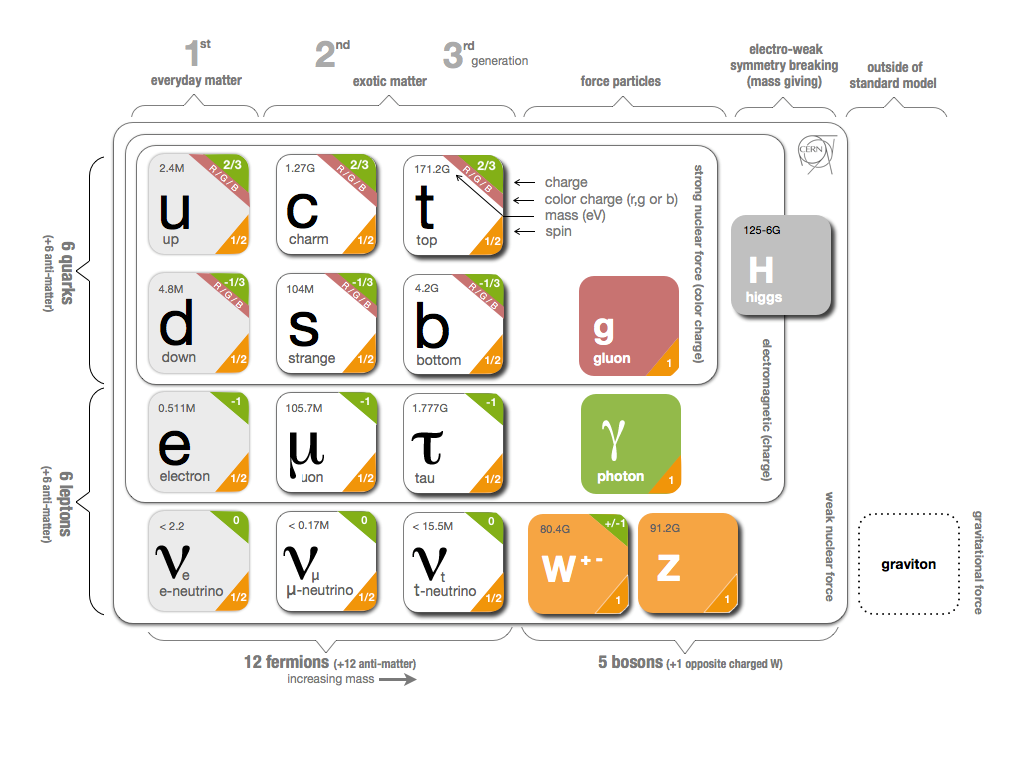
\includegraphics[width=6in]{images/SMinfographic_image}
    \caption[Standard Model Infographic]{An infographic of the Standard Model \cite{Purcell:1473657}. The elementary particles are arranged in their usual generational pairs and the surrounding solid lines divide them into sections based on the fundamental forces they experience.}
    \label{fig:SM}
\end{figure}

\subsection{Fermions}

The fermions encompass all forms of ordinary and exotic matter and obey Fermi-Dirac statistics because of their half-integer spin, namely, spin-\ensuremath{\frac{1}{2}}. They are divided into \textit{leptons} and \textit{quarks}. The electrically charged leptons interact via the electromagnetic and weak nuclear forces and include the familiar \textit{electron} (\lepe), the \textit{muon} (\lepm), and the \textit{tau} (\lept). The charged leptons also have neutral counterparts (\lepne, \lepnm, \lepnt) known as \textit{neutrinos}, which interact solely via the weak nuclear force. The quarks, having both electric and color charge, interact via the electromagnetic and strong and weak nuclear forces and include the up (\qrku), down (\qrkd), charm (\qrkc), strange (\qrks), bottom (\qrkb), and top (\qrkt). Although the leptons can exist freely, the nature of the strong interaction gives rise to color confinement, whereby quarks only appear within composite particles called hadrons. The bound states of quark doublets are known as mesons while those of quark triplets, of which the familiar proton is an example, are known as baryons.

The leptons and quarks are each arranged into pairs by flavour quantum number and sorted into three generations of increasing mass\footnote{The observation of neutrino oscillations disproved the prediction that they are massless but its implications for the lepton generations are unclear.}, as depicted in Figure \ref{fig:SM}. The more massive particles of the higher generations decay into the stable particles of the first generation, which corroborates the observation that ordinary matter consists of electrons and up and down quarks which are bound in protons and neutrons. There are no known constraints on the number of fermion generations, although experimental results suggest there are only three.

\subsection{Bosons}

The bosons, which obey Bose-Einstein statistics because of their integer spin, are divided into vector and scalar bosons. The spin-1 vector, or gauge, bosons mediate the fundamental forces and are exchanged between elementary particles during their interactions. The photon (\bosg) mediates the electromagnetic force, which is responsible for the phenomenon of intermolecular repulsion.\footnote{It is this repulsion that prevents us from passing through objects.} The \bosW\ and \bosZ\ bosons mediate the weak nuclear force that causes nuclear decay. And finally, the gluons (\bosgln) mediate the strong nuclear force that binds quarks into hadrons and even protons and neutrons in nuclei. The only spin-0 scalar boson in the theory is the Higgs boson (\bosH), which is responsible for the masses of the heavy gauge bosons and fermions.

\subsection{The Higgs Mechanism}

The requirement of gauge invariance under \symWEAK\ leads to a prediction of massless gauge bosons, which stands in contrast to the observation that the weak vector bosons are massive. In order to reconcile this observation while preserving the gauge invariance of the interaction, a mechanism of \textit{spontaneous symmetry breaking} was incorporated into the unified electroweak theory proposed by Sheldon Glashow \cite{EWKGLASHOW}, Abdus Salam \cite{EWKSALAM}, and Steven Weinberg \cite{EWKWEINBERG}. This mechanism, which came to be known as the \textit{Higgs mechanism}, was independently developed by Robert Brout and Fran\c{c}ois Englert \cite{HIGGSBE}, its namesake Peter Higgs \cite{HIGGSH}, and Gerald Guralnik, Richard Hagen, and Sir Thomas Kibble \cite{HIGGSGHK}.

The mechanism introduces into the Standard Model a scalar field $\phi$ represented as a complex doublet
\begin{equation}
  \phi = \begin{pmatrix}
           \phi^{+} \\
           \phi^{0} \\
         \end{pmatrix}
       = \frac{1}{\sqrt{2}}
         \begin{pmatrix}
           \phi_{1} + i\phi_{2} \\
           \phi_{3} + i\phi_{4} \\
         \end{pmatrix}
\end{equation}
and its potential $V(\phi)$ of the form
\begin{equation}
V(\phi) = \mu^{2}\phi^{\dag}\phi + \frac{\lambda}{2}(\phi^{\dag}\phi)^{2},
\end{equation}
where the real parameters $\mu^{2}$ and $\lambda$ represent the mass and self-coupling, respectively. The self-coupling $\lambda$ is taken to be positive by convention such that the potential is bounded from below. When $\mu^{2} > 0$, the potential is parabolic in shape and the ground state of the vacuum is at $\phi = 0$, keeping its symmetries intact. However, when $\mu^{2} < 0$, the minimum of the potential is no longer at $\phi = 0$ but rather\footnote{The solution is unique up to a phase $e^{i\theta}$, but it is customary to take $\theta = 0$.}
\begin{equation}
  v = \left(\frac{-\mu^{2}}{\lambda}\right)^{1/2},
  \label{eq:vev}
\end{equation}
where the vacuum now attains an expectation value $v$ in its ground state. The shape of such a potential is illustrated in Figure \ref{fig:potential}. The Higgs mechanism thus provides the means to spontaneously break the $\symWEAK \times \symEM$ symmetry within the model.

\begin{figure}[htbp]
  \centering
    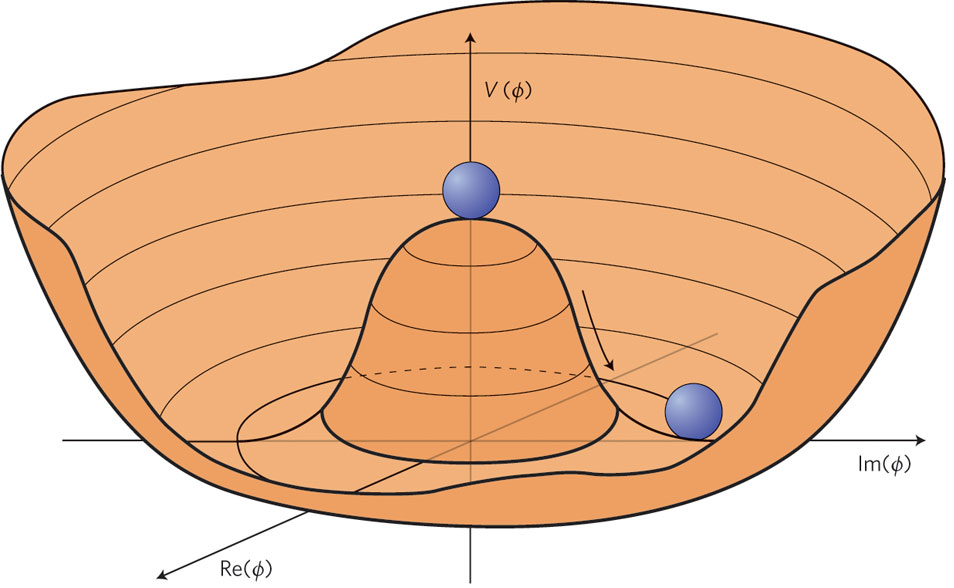
\includegraphics[width=3.5in]{images/higgspotential}
    \caption[Shape of the Higgs Field Potential]{The shape of the Higgs field potential for $\mu^{2} < 0$ \cite{deBoer:2013pud}. The transition of the field from its unstable state at the origin to its true ground state spontaneously breaks the rotational symmetry of the system.}
    \label{fig:potential}
\end{figure}

Because particles are excitations of their fields, the presence of the Higgs field also suggests the existence of the Higgs boson. An expression for the mass of this new boson can be determined by expanding the potential around the vacuum ground state $\phi_{0}$. By choosing the unitary gauge, the components of $\phi_{0}$ become
\begin{equation}
  (\phi_{1})_{0} = 0, (\phi_{2})_{0} = 0, (\phi_{3})_{0} = v, (\phi_{4})_{0} = 0
\end{equation}
and $\phi_{0}$ becomes simply
\begin{equation}
  \phi_{0} = \begin{pmatrix}
               \phi^{+} \\
               \phi^{0} \\
             \end{pmatrix}_{0}
           = \frac{1}{\sqrt{2}}
             \begin{pmatrix}
               0 \\
               v \\
             \end{pmatrix}.
\end{equation}
Then for small fluctuations $\phi(x) = \phi_{0} + H(x)$, the potential to second order in $H$ becomes
\begin{align}
  \begin{split}
    V(\phi) &= \frac{\mu^{2}}{2}(v^{2} + 2vH + H^{2}) + \frac{\lambda}{4}(v^{2} + 2vH + H^{2})^{2} \\
            &= \frac{1}{2}(\mu^{2}v^{2} + \frac{\lambda}{2}v^{4}) + (\mu^{2}v + \lambda v^{3})H + \frac{1}{2}(\mu^{2} + 3\lambda v^{2})H^{2} + \mathcal{O}(H^{3}) \\
            &= V_{0} - \frac{1}{2}(2\mu^{2})H^{2} + \mathcal{O}(H^{3}), \\
  \end{split}
  \label{eq:higgsexpand}
\end{align}
where $V_{0}$ collects the constant terms and Equation \ref{eq:vev} has been used to vanish the first order term and simplify the second order term. The mass can be read from the coefficient of the second order term in $H$:
\begin{equation}
  m_{H}^{2} = -2\mu^{2} \implies m_{H} = \sqrt{2}\mu = \sqrt{2\lambda}v,
\end{equation}
where the sign of the mass was dropped because $\mu^2$ was chosen to be negative. Although the Standard Model predicts a massive Higgs boson, its dependence on the value of the unknown self-coupling parameter $\lambda$ and the vacuum expectation value $v$ means it must be determined experimentally.

\subsubsection{Gauge boson masses}

The necessity of the Higgs mechanism is realized by how it generates the masses of the gauge bosons. The Lagrangian for the Higgs may be written as
\begin{equation}
  \mathcal{L}_{\phi} = (D_{\mu}\phi)^{\dag}(D^{\mu}\phi) - V(\phi) = (D_{\mu}\phi)^{\dag}(D^{\mu}\phi) - \mu^{2}\phi^{\dag}\phi - \frac{\lambda}{2}(\phi^{\dag}\phi)^{2},
  \label{eq:Lhiggs}
\end{equation}
By definition, the Higgs field has weak hypercharge $Y = +1$ and weak isospin $T_{3} = -1/2$. The weak hypercharge $Y$ and weak isospin $T$ are the generators of the \symWEAK\ and \symEM\ symmetries, respectively, with the choice of their values made to satisfy the relation
\begin{equation}
  Q = T_{3} + \frac{1}{2}Y,
\end{equation}
where $Q$ is the electric charge.\footnote{Hence, the Higgs boson is a neutral particle.} These choices require the covariant derivative of the kinetic term to be of the form
\begin{equation}
  D_{\mu}\phi = (\partial_{\mu} - \frac{i}{2}g\boldsymbol\sigma\cdot\mathbf{W}_{\mu} - \frac{i}{2}g^{\prime}B_{\mu})\phi,
\end{equation}
where $\mathbf{W_{\mu}}$ and $B_{\mu}$ are, respectively, the \symWEAK\ and \symEM\ gauge bosons, $g$ and $g^{\prime}$ are the corresponding gauge couplings, and $\boldsymbol\sigma = \sigma^{a}, a = 1, 2, 3$ are the Pauli matrices.

The gauge boson masses are contained in the kinetic term of the Lagrangian and can be determined by evaluating its expression for the vacuum ground state. The covariant derivative becomes
\begin{align}
  \begin{split}
    D_{\mu}\phi &\rightarrow \left[ \partial_{\mu} - \frac{i}{2}g \begin{pmatrix} W_{\mu}^{3} & W_{\mu}^{1} - iW_{\mu}^{2} \\ W_{\mu}^{1} + iW_{\mu}^{2} & -W_{\mu}^{3} \\ \end{pmatrix} - \frac{i}{2}g^{\prime}B_{\mu} \right] \frac{1}{\sqrt{2}} \begin{pmatrix} 0 \\ v + H \\ \end{pmatrix} \\[1em]
                &= -\frac{i}{2} \begin{pmatrix} \frac{g}{\sqrt{2}}(W_{\mu}^{1}-iW_{\mu}^{2})(v + H) \\ i\sqrt{2}\partial_{\mu}H + \frac{1}{\sqrt{2}}(-gW_{\mu}^{3} + g^{\prime}B_{\mu})(v + H) \\ \end{pmatrix} \\
  \end{split}
\end{align}
and substituting this expression into Equation \ref{eq:Lhiggs} while ignoring the potential term for clarity yields
\begin{align}
  \begin{split}
    \mathcal{L}_{\phi} &= \frac{1}{4} \begin{vmatrix} \frac{g}{\sqrt{2}}(W_{\mu}^{1}-iW_{\mu}^{2})(v + H) \\ i\sqrt{2}\partial_{\mu}H + \frac{1}{\sqrt{2}}(-gW_{\mu}^{3} + g^{\prime}B_{\mu})(v + H) \\ \end{vmatrix}^{2} \\[1em]
                       &= \frac{1}{4} \left[ 2(\partial_{\mu}H)^{2} + \left( \frac{g^{2}}{2} \left( (W_{\mu}^{1})^{2} + (W_{\mu}^{2})^{2} \right) + \frac{1}{2} \left( g^{\prime}B_{\mu} - gW_{\mu}^{3} \right)^{2} \right) (v + H)^{2} \right] \\[1em]
                       &= \frac{1}{2}(\partial_{\mu}H)^{2} + \frac{g^{2}}{8}(W_{\mu}^{1})^{2}v^{2} + \frac{g^{2}}{8}(W_{\mu}^{2})^{2}v^{2} + \frac{1}{8}\left( g^{\prime}B_{\mu} - gW_{\mu}^{3} \right)^{2}v^{2} + \mathcal{O}(H), \\
    \label{eq:gaugemasses}
  \end{split}
\end{align}
where higher order terms in $H$ have been discarded. The result of Equation \ref{eq:gaugemasses} reveals that the broken symmetry of the Higgs field causes the $W_{\mu}^{1}$ and $W_{\mu}^{2}$ vector fields to both acquire a mass of
\begin{equation}
  m_{W}^{2} = \frac{g^{2}v^{2}}{4} \implies m_{W} = \frac{gv}{2}.
\end{equation}
The linear combination of vector fields $(g^{\prime}B_{\mu} - gW_{\mu}^{3})$ also acquires a mass that depends on the couplings $g$ and $g^{\prime}$, and is typically expressed as
\begin{equation}
  m_{Z}^{2} = \frac{(g^{2} + g^{\prime 2}) v^{2}}{4} \implies m_{Z} = \frac{\sqrt{g^{2} + g^{\prime 2}} v}{2}.
\end{equation}
The excitations of these massive vector fields are the weak gauge bosons \bosWp, \bosWm, and \bosZn\ which have been observed in nature and whose masses have been measured\cite{PDG2018} to be
\begin{equation}
  m_{\bosWp} = m_{\bosWm} = 80.379 \pm 0.012\ \GeV\ \mathrm{and}\ m_{\bosZn} = 91.1876 \pm 0.0021\ \GeV.
\end{equation}

The derivation would be complete but for a missing gauge boson. Recall our earlier transformation to the unitary gauge which fixed three of the four degrees of freedom of the Higgs field. According to Goldstone's Theorem\cite{Goldstone}, these degrees of freedom become the longitudinal polarizations of the now massive weak gauge bosons. The untouched degree of freedom thus corresponds to the massless photon \bosg. By taking the electromagnetic field $A_{\mu}$ to be proportional to the missing linear combination of fields $(g^{\prime}W_{\mu}^{3} + gB_{\mu})$, it can be explicitly introduced into the kinetic term of the Lagrangian while remaining orthogonal to the other fields.

\subsubsection{Fermion masses}

Although the Dirac Lagrangian describes the dynamics of the fermions, it is inadequate for explaining their observed masses. This is because a Dirac mass term of the form
\begin{equation}
  m\bar{\psi}\psi = m(\bar{\psi}_{L} + \bar{\psi}_{R})(\psi_{L} + \psi_{R}) = m(\bar{\psi}_{L}\psi_{R} + \bar{\psi}_{R}\psi_{L})
\end{equation}
violates the gauge invariance of the model by coupling together left-handed and right-handed fermions which transform differently under both \symWEAK\ and \symEM. The masses of the fermions are instead another consequence of spontaneous symmetry breaking, and their coupling to the scalar Higgs field through Yukawa interactions gives rise to their mass terms in the Standard Model Lagrangian.

The Yukawa interaction of the first generation leptons to the Higgs field $\phi$ is given by
\begin{equation}
  \mathcal{L}_{\mathrm{Yukawa}} = -\lambda_{\lepe} \left( \bar{L} \phi \lepe_{R} + \lepebar_{R} \phi^{\dag} L\right),
\end{equation}
where $\lambda_{\lepe}$ is the coupling constant, the \symWEAK\ singlet $\lepe_{R}$ represents the right-handed electron, and the \symWEAK\ doublet $L$ represents the left-handed neutrino\footnote{The neutrinos have been experimentally measured, within uncertainties, to have left-handed helicity only.} and electron, i.e.
\begin{equation}
  L = \begin{pmatrix} \nu_{L} \\ \lepe_{L} \\ \end{pmatrix}.
\end{equation}
Evaluating this expression for the vacuum ground state yields the electron mass term
\begin{align}
  \begin{split}
    \mathcal{L}_{\mathrm{Yukawa}} &= -\lambda_{\lepe} \left( \bar{L} \phi_{0} \lepe_{R} + \lepebar_{R} \phi_{0}^{\dag} L\right) \\[1em]
                                  &= -\frac{\lambda_{\lepe}}{\sqrt{2}} \left[ \begin{pmatrix} \bar{\nu}_{L} & \lepebar_{L} \\ \end{pmatrix} \begin{pmatrix} 0 \\ v \\ \end{pmatrix}_{0} \lepe_{R} + \lepebar_{R} \begin{pmatrix} 0 & v \\ \end{pmatrix}_{0} \begin{pmatrix} \nu_{L} \\ \lepe_{L} \\ \end{pmatrix} \right] \\[1em]
                                  &= -\frac{\lambda_{\lepe}v}{\sqrt{2}} \left( \lepebar_{L} \lepe_{R} + \lepebar_{R} \lepe_{L} \right), \\[1em]
  \end{split}
\end{align}
which gives the electron mass
\begin{equation}
  m_{\lepe} = \frac{\lambda_{\lepe}v}{\sqrt{2}}.
\end{equation}
Therefore the electron, and similarly for the charged leptons of the other generations, is a mixture of left-handed and right-handed fields which acquire a mass that is proportional to the vacuum expectation value $v$ and their coupling to the Higgs field.

The Yukawa interaction of the quarks, taking into account the existence of the right-handed \symWEAK\ singlet $\qrku_{R}$, is similarly given by
\begin{equation}
  \mathcal{L}_{\mathrm{Yukawa}} = -\Lambda_{\qrkd}^{ij} \left( \bar{Q}_{L}^{i} \phi \qrkd_{R}^{j} + \qrkdbar_{R}^{j} \phi^{\dag} Q_{L}^{i} \right) -\Lambda_{\qrku}^{ij} \left( \bar{Q}_{L}^{i} \tilde{\phi} \qrku_{R}^{j} + \qrkubar_{R}^{j} \tilde{\phi}^{\dag} Q_{L}^{i} \right),
\end{equation}
where $\Lambda_{\qrkd}^{ij}$ and $\Lambda_{\qrku}^{ij}$ are $3 \times 3$ complex matrices of couplings for the down-type and up-type quarks, respectively, whose indices $i$ and $j$ run over the quark generations, $\qrkd_{R}$ and $\qrku_{R}$ are the right-handed singlets, $Q_{L}$ is the left-handed doublet
\begin{equation}
  Q_{L} = \begin{pmatrix} u_{L} \\ d_{L} \\ \end{pmatrix},
\end{equation}
and $\tilde{\phi}$ is the charge conjugate of the Higgs doublet
\begin{equation}
  \tilde{\phi} = \begin{pmatrix} \phi^{0*} \\ -\phi^{+*} \\ \end{pmatrix} \implies \tilde{\phi}_{0} = \begin{pmatrix} v \\ 0 \\ \end{pmatrix}.
\end{equation}
Proceeding as before, evaluating this expression for the vacuum ground state yields
\begin{equation}
  \mathcal{L}_{\mathrm{Yukawa}} = -\frac{v}{\sqrt{2}} \Lambda_{\qrkd}^{ij} \left( \qrkdbar_{L}^{i} \qrkd_{R}^{j} + \qrkdbar_{R}^{j} \qrkd_{L}^{i} \right) -\frac{v}{\sqrt{2}} \Lambda_{\qrku}^{ij} \left( \qrkubar_{L}^{i}\qrku_{R}^{j} + \qrkubar_{R}^{j} \qrku_{L}^{i} \right),
\end{equation}
from which the quark masses are found to be
\begin{equation}
  M_{\qrkd}^{ij} = \frac{\Lambda_{\qrkd}^{ij}v}{\sqrt{2}}\ \mathrm{and}\ M_{\qrku}^{ij} = \frac{\Lambda_{\qrku}^{ij}v}{\sqrt{2}}.
\end{equation}
These mass terms resemble those of leptons except that they are matrices which depend on the Yukawa couplings of the mixed quark states to the Higgs field. The physical quark fields correspond to the mass eigenstates obtained by diagonalizing the mass matrices $M_{\qrkd}^{ij}$ and $M_{\qrku}^{ij}$. A general complex matrix may be diagonalized by a biunitary transformation, so there exist unitary matrices $\mathbf{D}_{L}$, $\mathbf{D}_{R}$, $\mathbf{U}_{L}$, and $\mathbf{U}_{R}$ such that
\begin{equation}
  \mathbf{D}_{L}^{\dag}\mathbf{M}_{\qrkd}\mathbf{D}_{R} = \begin{pmatrix} m_{\qrkd} & 0 & 0 \\ 0 & m_{\qrks} & 0 \\ 0 & 0 & m_{\qrkb} \\ \end{pmatrix},\ \mathbf{U}_{L}^{\dag}\mathbf{M}_{\qrku}\mathbf{U}_{R} = \begin{pmatrix} m_{\qrku} & 0 & 0 \\ 0 & m_{\qrkc} & 0 \\ 0 & 0 & m_{\qrkt} \\ \end{pmatrix},
\end{equation}
where the mass eigenvalues are real and positive. But this transformation also amounts to diagonalizing the Yukawa coupling matrices, thus revealing that the quark masses also depend on their couplings and the vacuum expectation value in the same fashion as the charged leptons.

\section{The Higgs Boson}

While the Standard Model predicts the existence of the Higgs boson, it does not predict the value of its self-coupling $\lambda$ and therefore its mass \massH\ is an unknown parameter of the model. Theoretical constraints based on unitarity bounds, the stability of the vacuum, and the energy scale of Standard Model physics only place the value of \massH\ within a wide range from 100 \GeV\ up to 1 \TeV. Stronger limits on \massH\, not to mention an observation of the elusive boson, would have to be obtained from experimental results. During the 1980s, experimental searches for the Higgs boson began in earnest as particle accelerators finally reached energies that enabled the predicted mass range to be studied. The current era of high-energy physics experiment is now dominated by experiments at the Large Hadron Collider (LHC) and so the following qualitative review of Standard Model Higgs boson phenomenology is framed in its context.

\subsection{Phenomenology}

The Standard Model Higgs boson is predicted to be a spinless particle with zero electric or color charge that is even under the combined symmetry of charge conjugation and parity (CP-symmetry). It is also predicted to couple to the gauge bosons, fermions, and itself\footnote{The Higgs self-couplings come from the higher order terms of Equation \ref{eq:higgsexpand}.} in proportion to their masses according to
\begin{equation}
  \begin{array}{ccc}
    g_{Hf\bar{f}} = \frac{m_{f}}{v}, & g_{HVV} = \frac{2m_{V}^{2}}{v}, & g_{HHVV} = \frac{2m_{V}^{2}}{v^{2}}, \\[1em]
    g_{HHH} = \frac{3m_{H}^{2}}{v},  & g_{HHHH} = \frac{3m_{H}^{2}}{v^{2}}, \\
  \end{array}
\end{equation}
where $V = \bosW\ \mathrm{or}\ \bosZ$ and $v$ is the vacuum expectation value.\cite{PDG2018} These interactions may be expressed as the Feynman diagram vertices shown in Figure \ref{fig:higgsvertices}. Because the Higgs boson might be coaxed into existence by these interactions, the production modes of the Higgs boson have informed the development of modern hadron colliders. By the same token, those interactions provide the means for the massive Higgs boson to decay into lighter and more stable particles. The decay modes of the Higgs boson thus influence the design of particle detectors capable of accurately measuring the properties of its decays products.

\begin{figure}[htbp]
  \centering
  \mbox{
    \subfigure [] {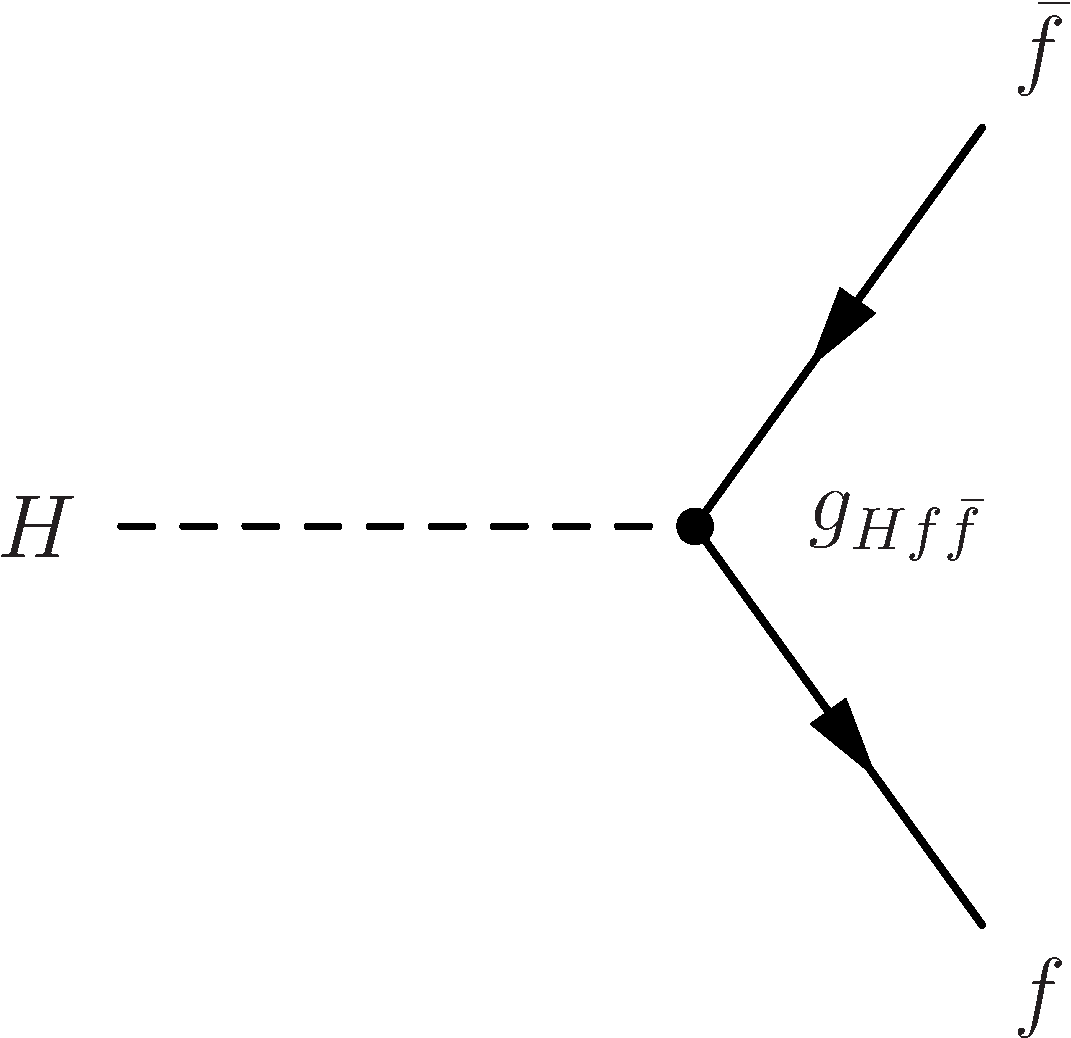
\includegraphics[scale=0.2]{images/vertex-Hff}} \qquad
    \subfigure [] {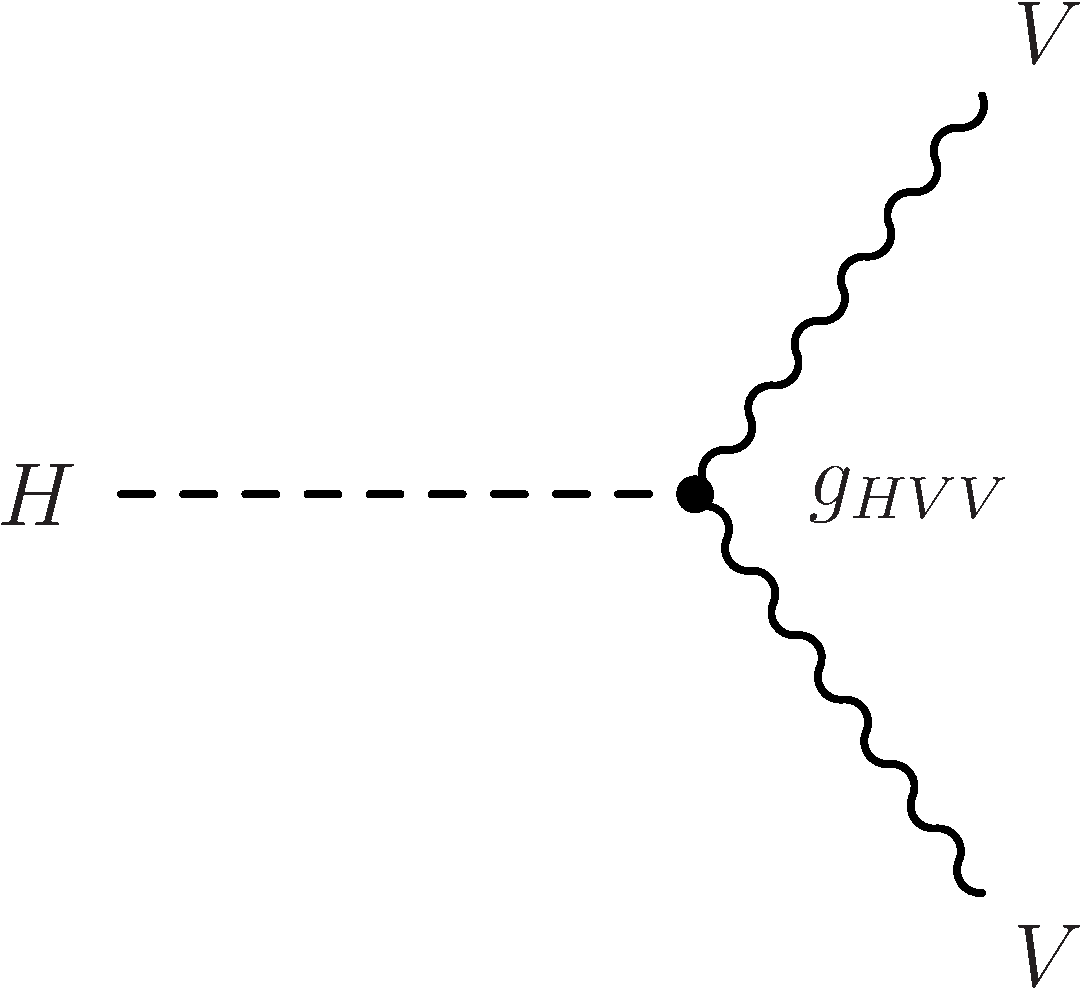
\includegraphics[scale=0.2]{images/vertex-HVV}} \qquad
    \subfigure [] {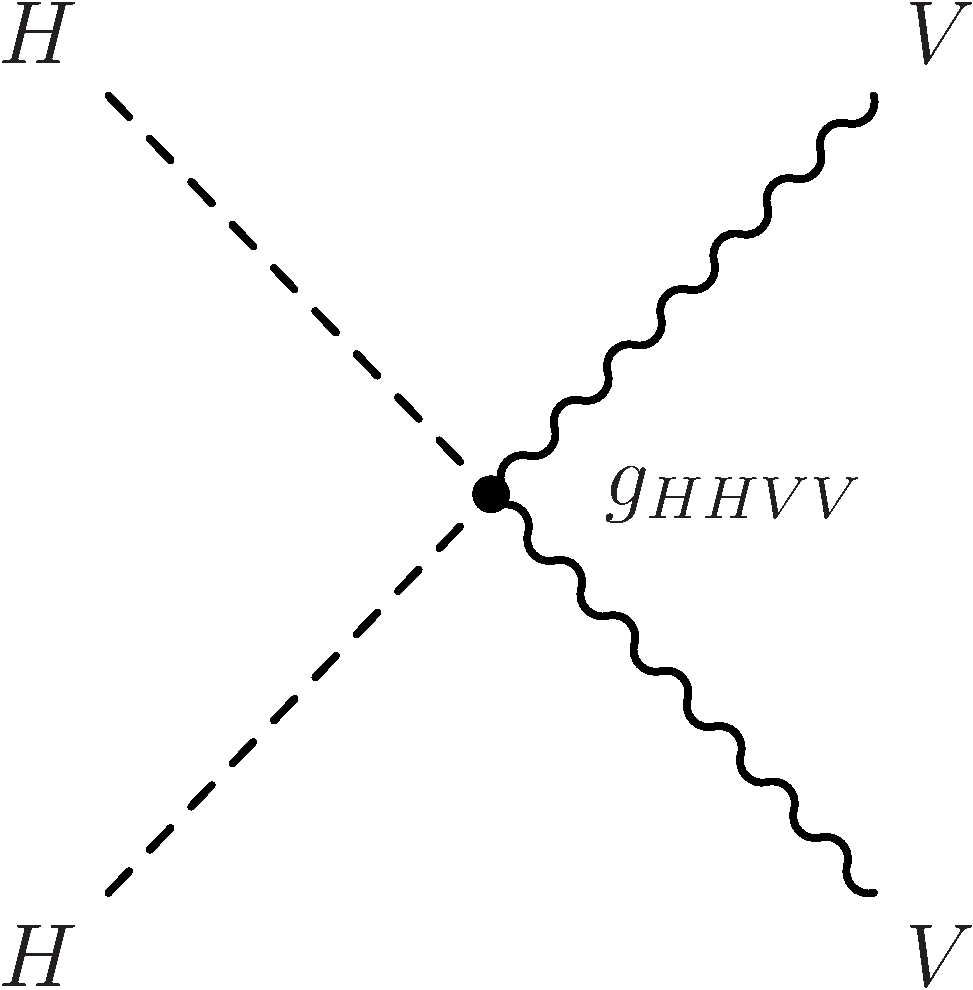
\includegraphics[scale=0.2]{images/vertex-HHVV}} \qquad
  }
  \mbox{
    \subfigure [] {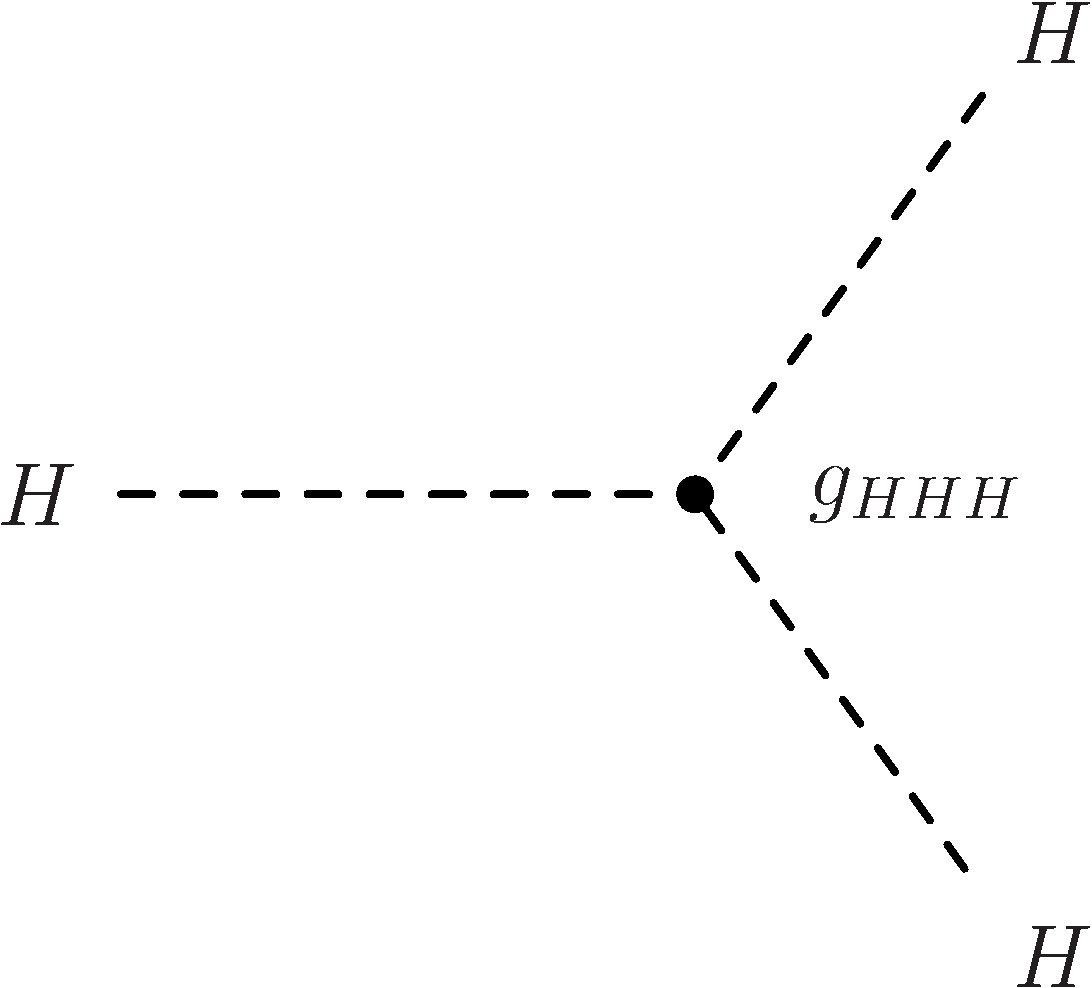
\includegraphics[scale=0.2]{images/vertex-HHH}} \qquad
    \subfigure [] {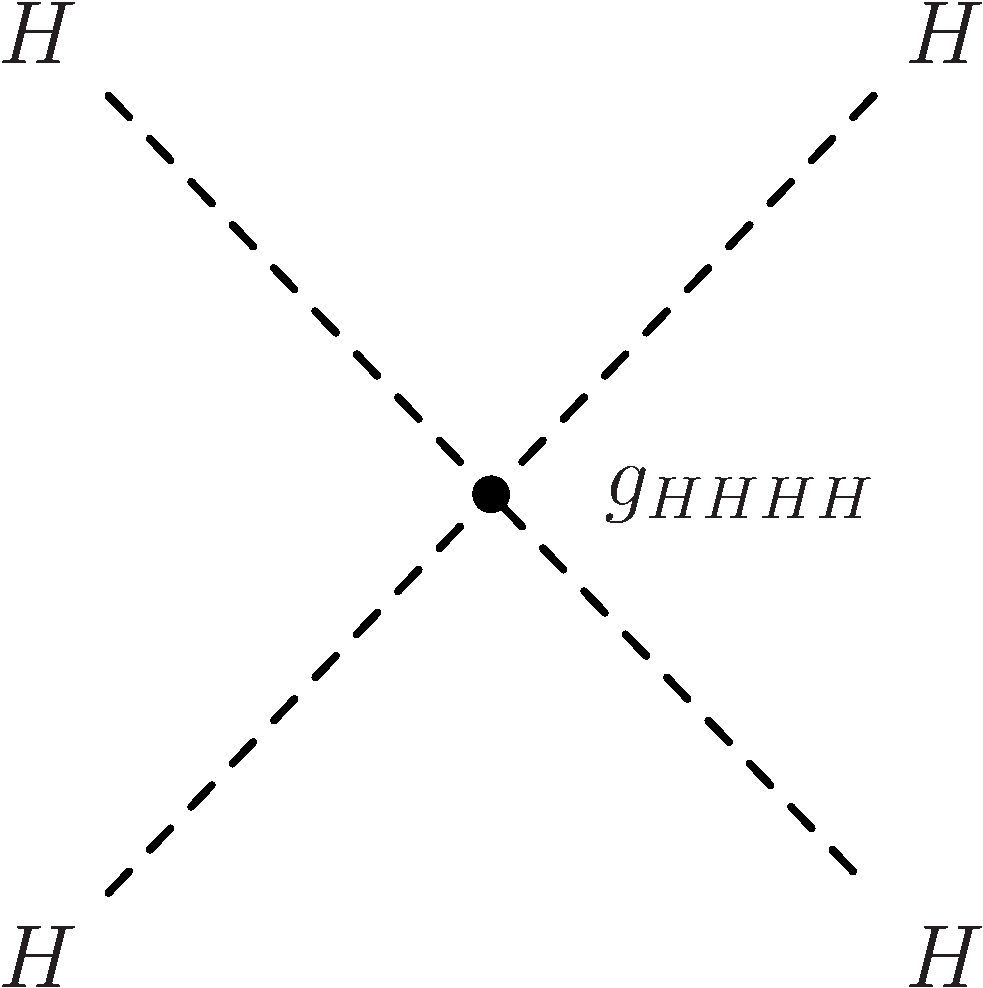
\includegraphics[scale=0.2]{images/vertex-HHHH}} \qquad
  }
  \caption[Higgs Boson Interaction Vertices]{The Feynman diagrams for the vertices of the Standard Model Higgs boson representing the A) fermion-Higgs interaction; B) trilinear gauge-Higgs interaction; C) quartic gauge-Higgs interaction; D) trilinear self-interaction; E) quartic self-interaction.}
  \label{fig:higgsvertices}
\end{figure}
 
\subsubsection{Production Modes}

The production of massive particles such as the Higgs boson proceeds from the interactions of hadrons made to collide at high energies. The probability that such a collision results in a specific interaction is known as a cross section $\sigma$. The production cross sections of the Higgs boson depend on the center-of-mass energy of the collision $\sqrt{s}$ and its mass \massH, and have been determined by theoretical calculations to behave as shown in Figure \ref{fig:higgsprodxsec}.

\begin{figure}[htbp]
  \centering
  \mbox{
    \subfigure [] {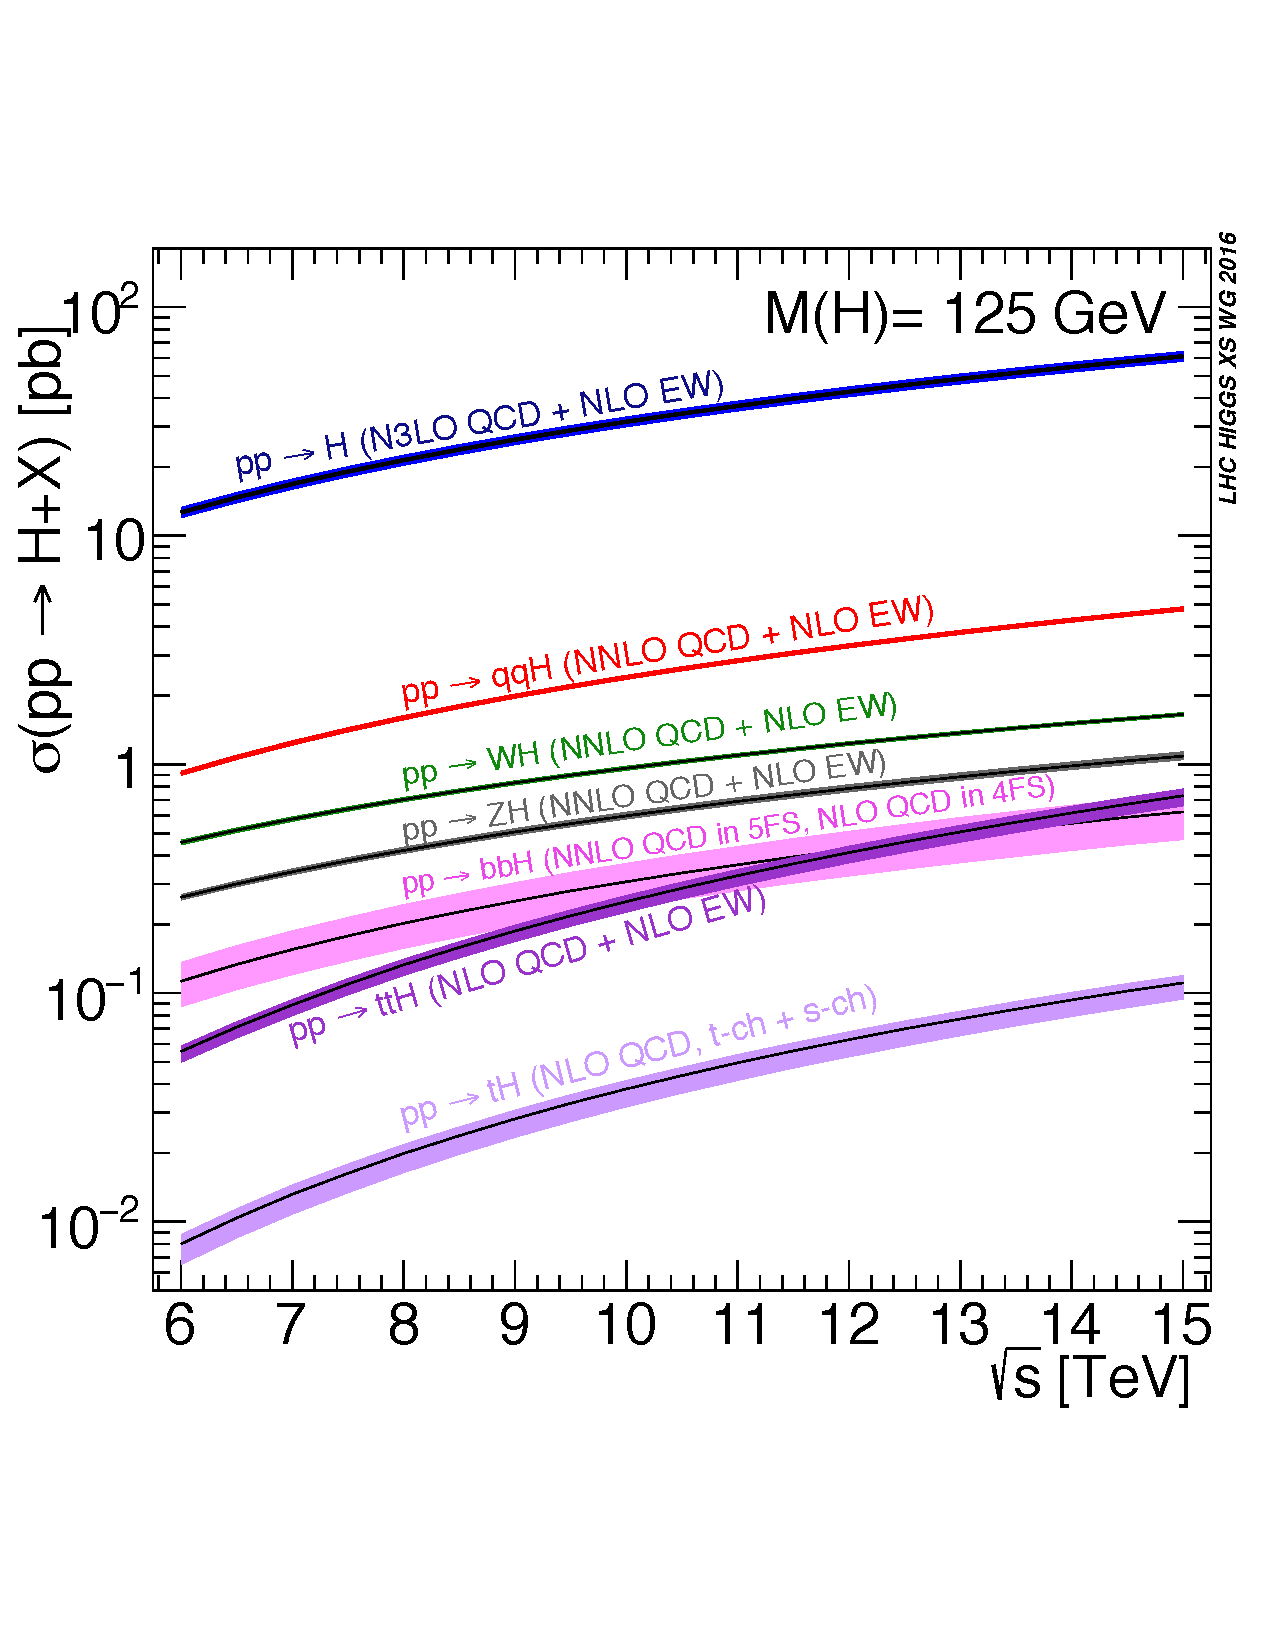
\includegraphics[scale=0.36]{images/Plot_Escan_H125_new_sqrt}} \qquad
    \subfigure [] {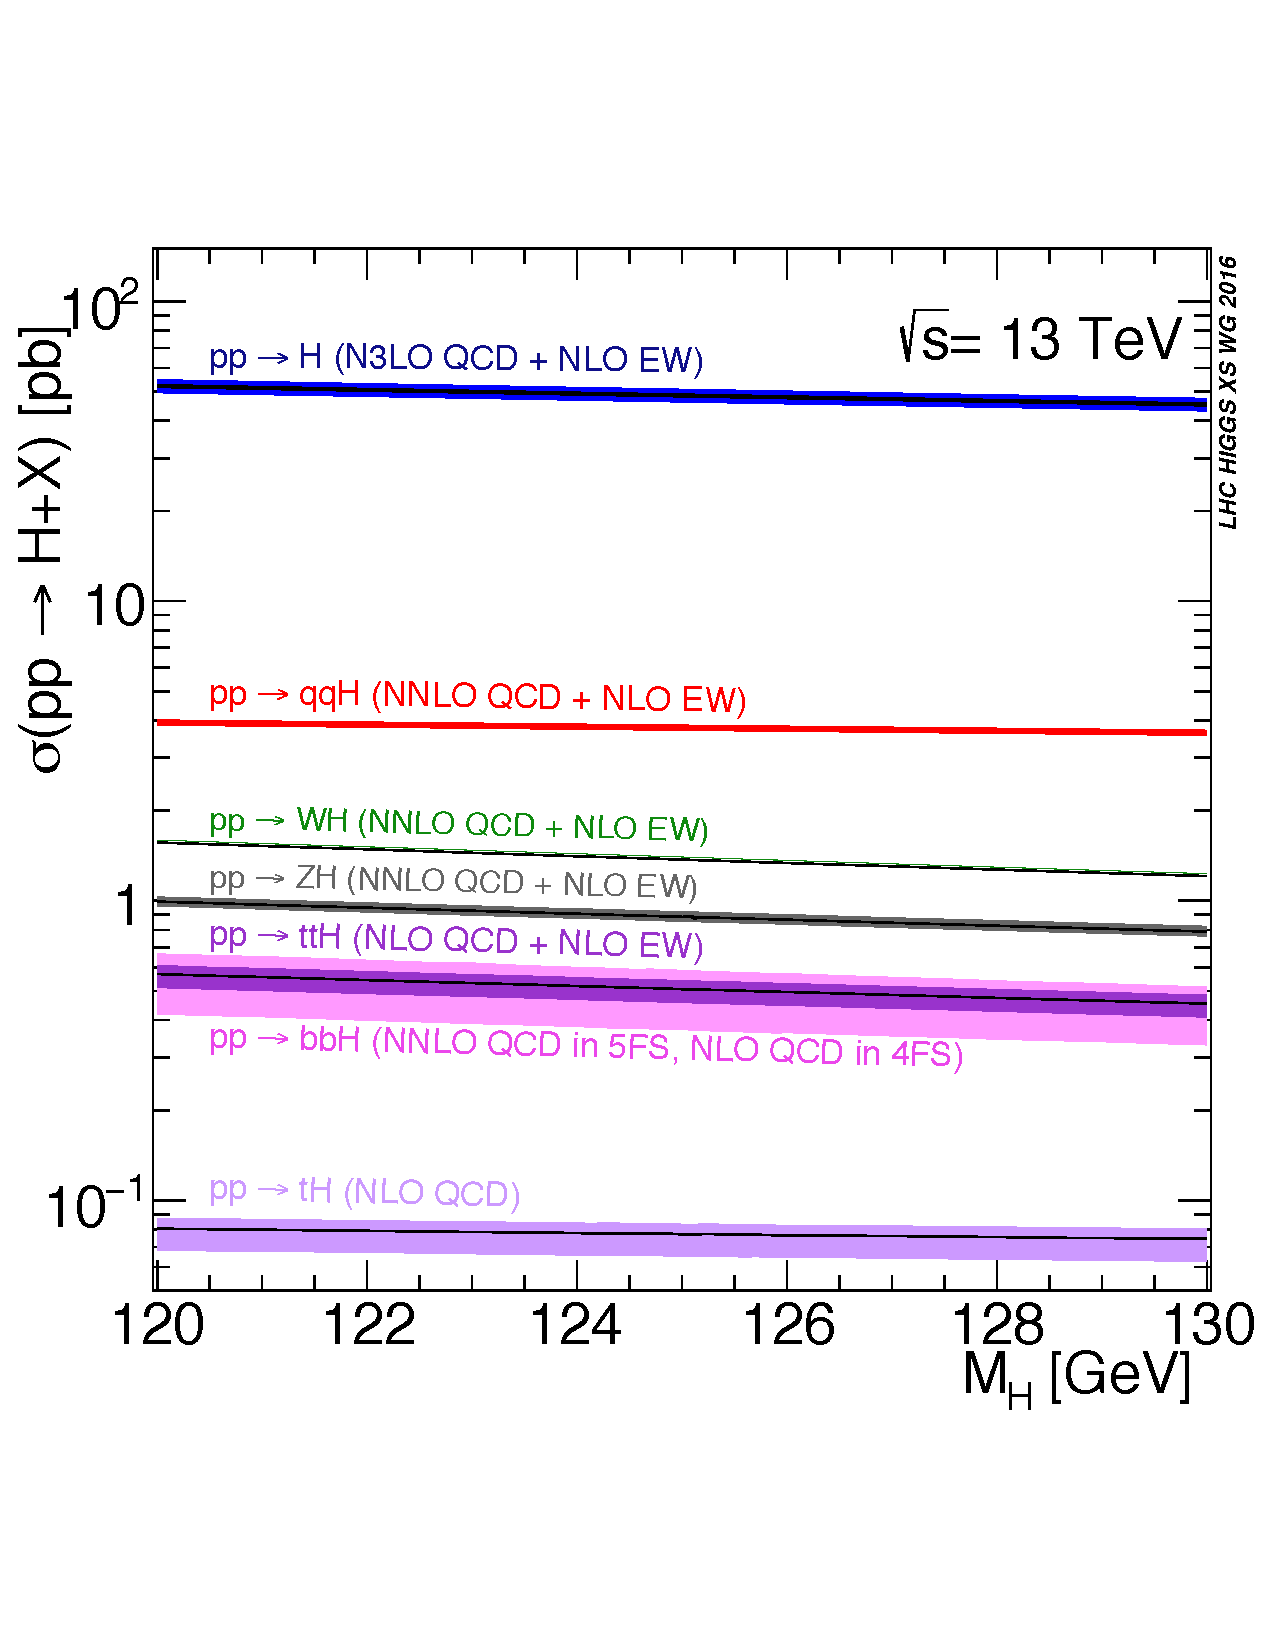
\includegraphics[scale=0.36]{images/plot_13tev_H_sqrt}} \qquad
  }
  \caption[Higgs Boson Production Cross Sections]{The production cross section for the Higgs boson as A) a function of the center of mass energy $\sqrt{s}$ for $\massH = 125\ \GeV$; B) a function of \massH\ for $\sqrt{s} = 13\ \TeV$. The shaded bands show the combined parametric and theoretical uncertainties and the labels indicate the production mode and any radiative corrections considered.\cite{CERNYR4}}
  \label{fig:higgsprodxsec}
\end{figure}

The dominant production mode is gluon fusion ($pp \rightarrow H$), in which a gluon from each of the colliding hadrons form a virtual quark loop. Because the Higgs boson couples to quarks in proportion to their masses, it can be radiated from the resulting virtual top quark or, to a lesser extent, bottom quark loop. The production mode with the second-largest cross section is vector boson fusion ($pp \rightarrow qqH$), which proceeds from the parton scattering of two quarks, or anti-quarks, via their exchange of weak vector bosons \bosV. This produces a Higgs boson because of the allowed the trilinear gauge-Higgs interaction. The vector boson associated production mode ($pp \rightarrow \VH$), or \textit{Higgstrahlung}, has the third-largest cross section. This production mechanism proceeds from the weak interaction of a quark and an anti-quark from which a Higgs boson is radiated by the virtual \bosW\ or \bosZ\ weak vector boson. Because the \bosZ\ associated production can also be induced via a virtual top quark loop, contributions of nearly 15\% to the total production cross section of this mode come from the process $\bosgln\bosgln \rightarrow \bosZ\bosH$. The fourth relevant production mode is top quark pair associated production ($pp \rightarrow ttH$). Rather than forming a virtual top quark loop, a gluon from each of the colliding hadrons decays into a top quark-antiquark pair and a Higgs boson is produced by the annhiliation of a top quark of one pair and the top anti-quark of the other. The smallest cross sections are contributed by the single top quark associated production and bottom quark pair associated production modes, which are suppressed relative to the main production modes. The Feynman diagrams for the main production modes are shown in Figure \ref{fig:higgsprodfeyn}.

\begin{figure}[htbp]
  \centering
  \mbox{
    \subfigure [] {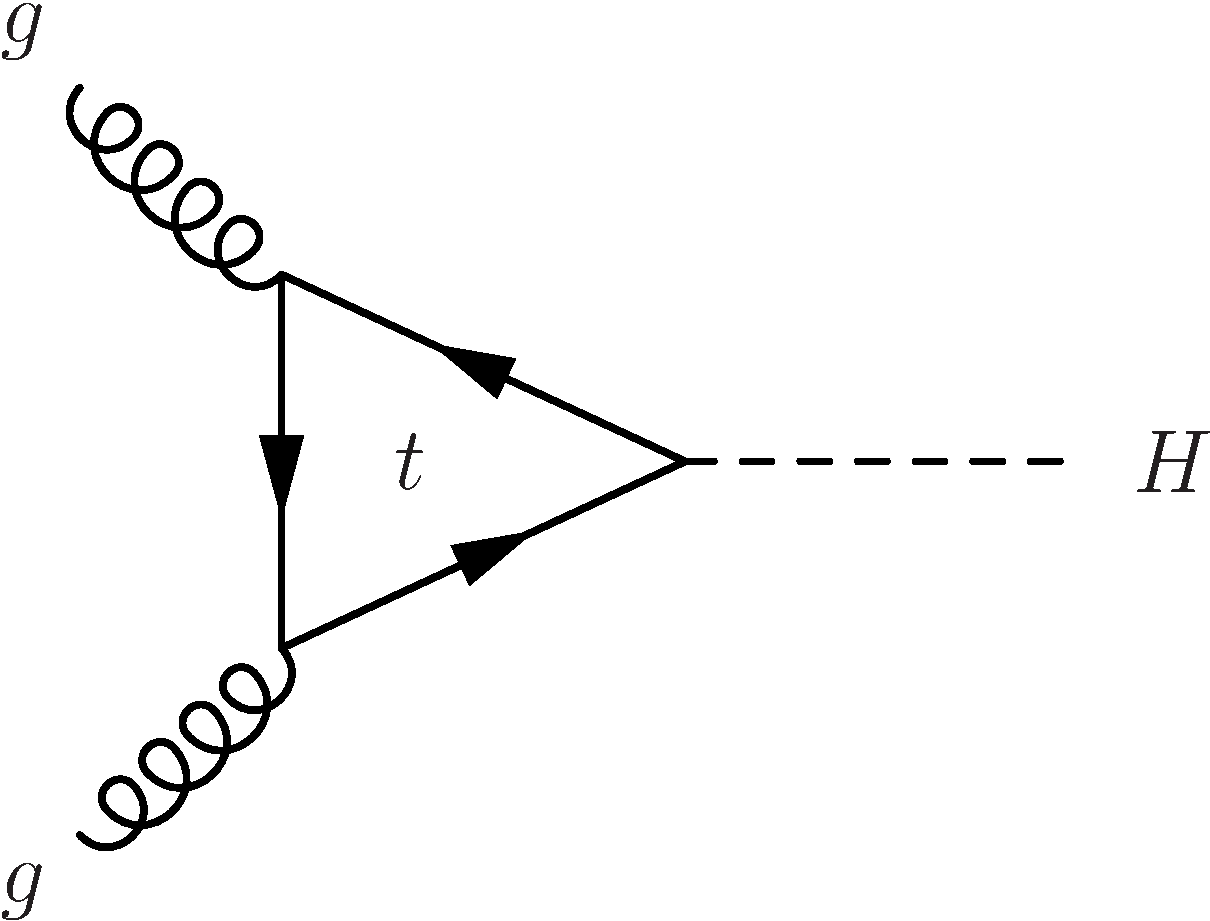
\includegraphics[scale=0.2]{images/production-ggH}} \qquad
    \subfigure [] {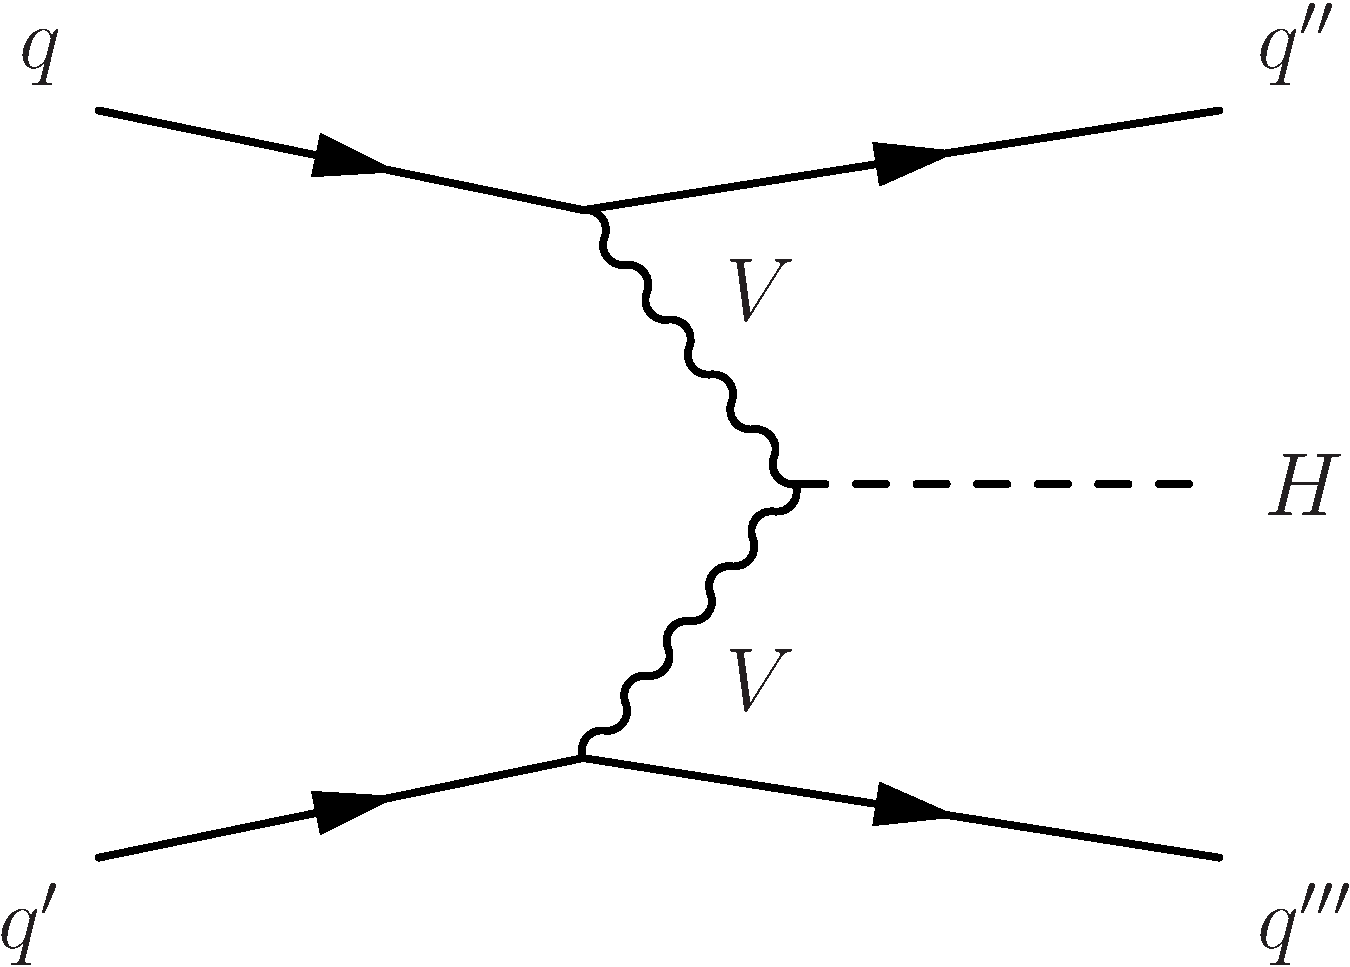
\includegraphics[scale=0.2]{images/production-VBF}} \qquad
    \subfigure [] {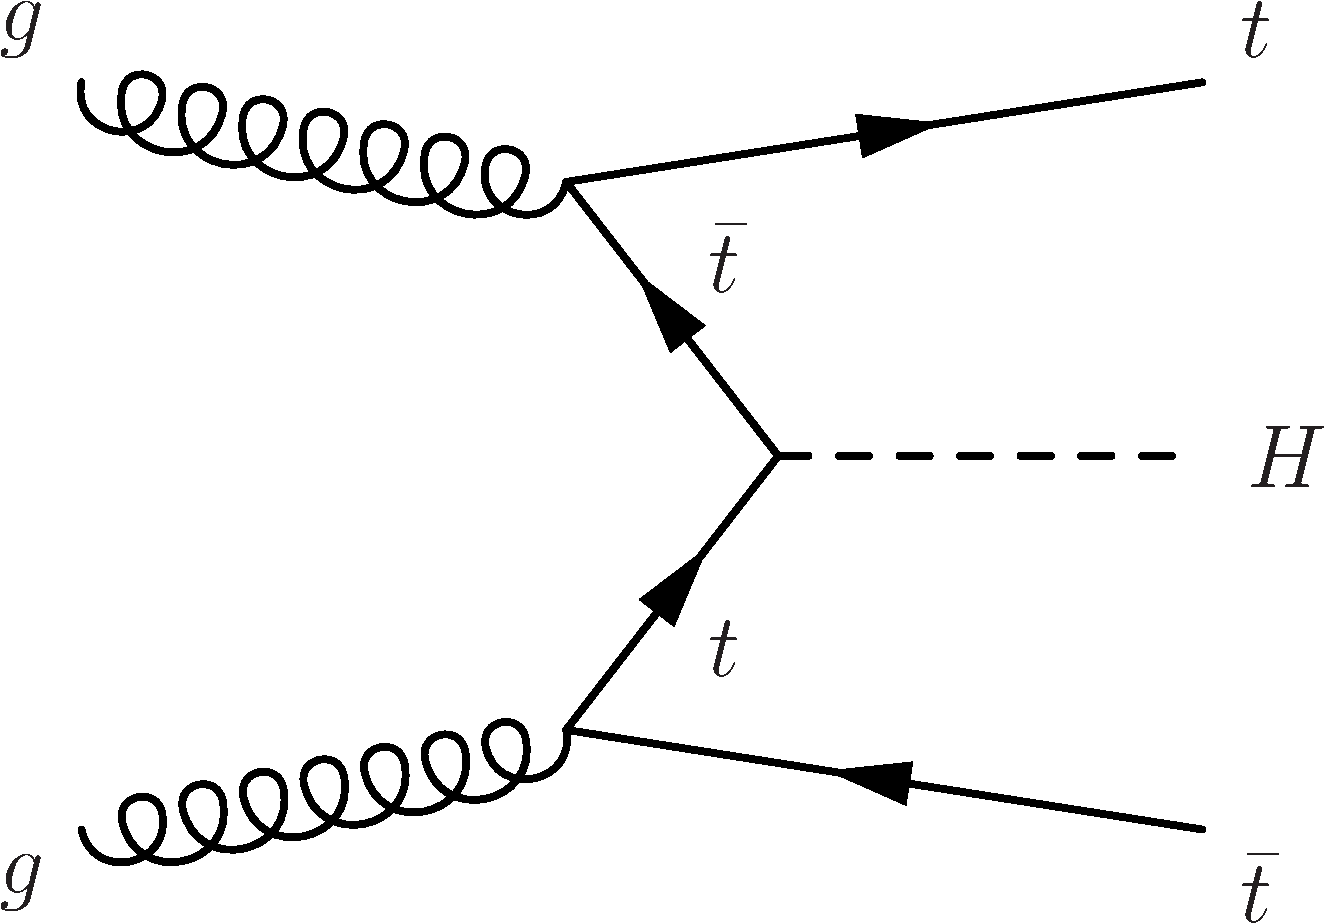
\includegraphics[scale=0.2]{images/production-ttH}} \qquad
  }
  \mbox{
    \subfigure [] {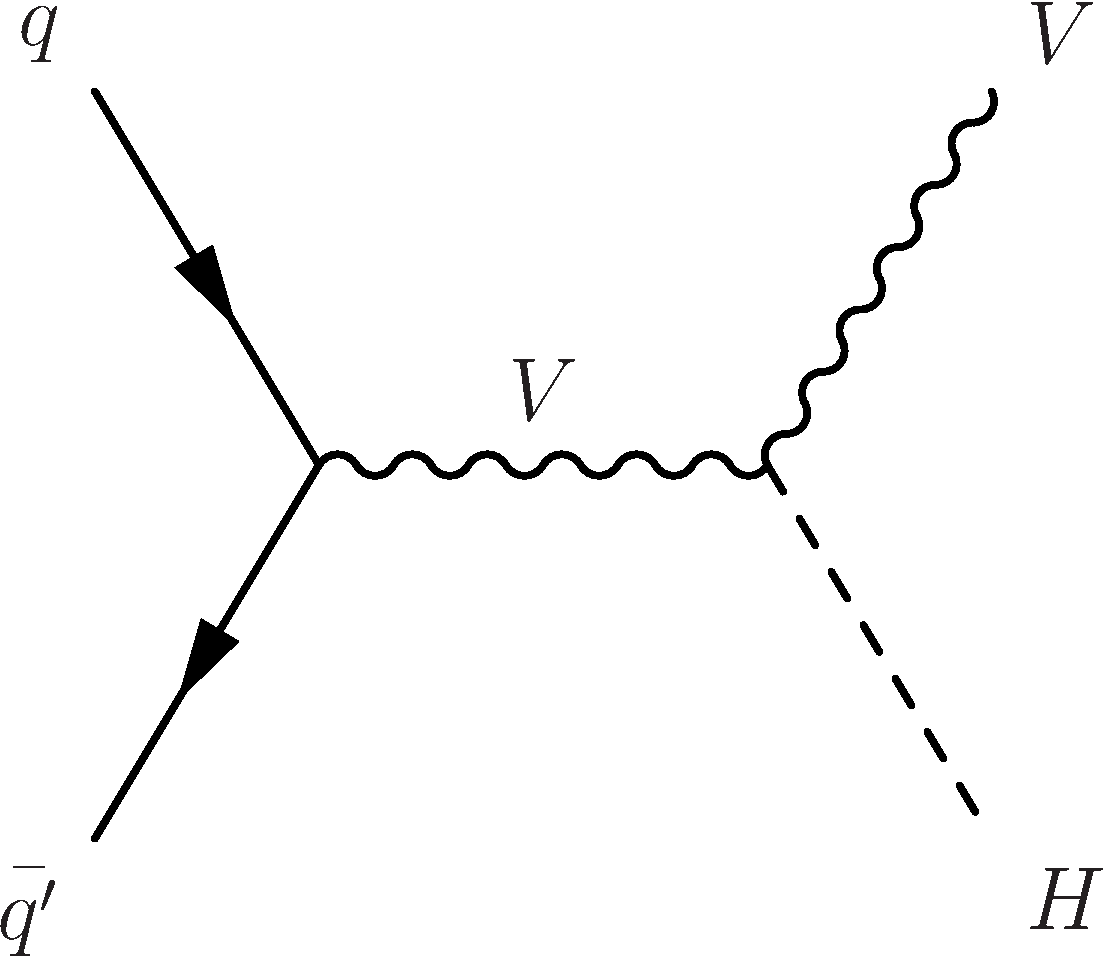
\includegraphics[scale=0.2]{images/production-VH}} \qquad
    \subfigure [] {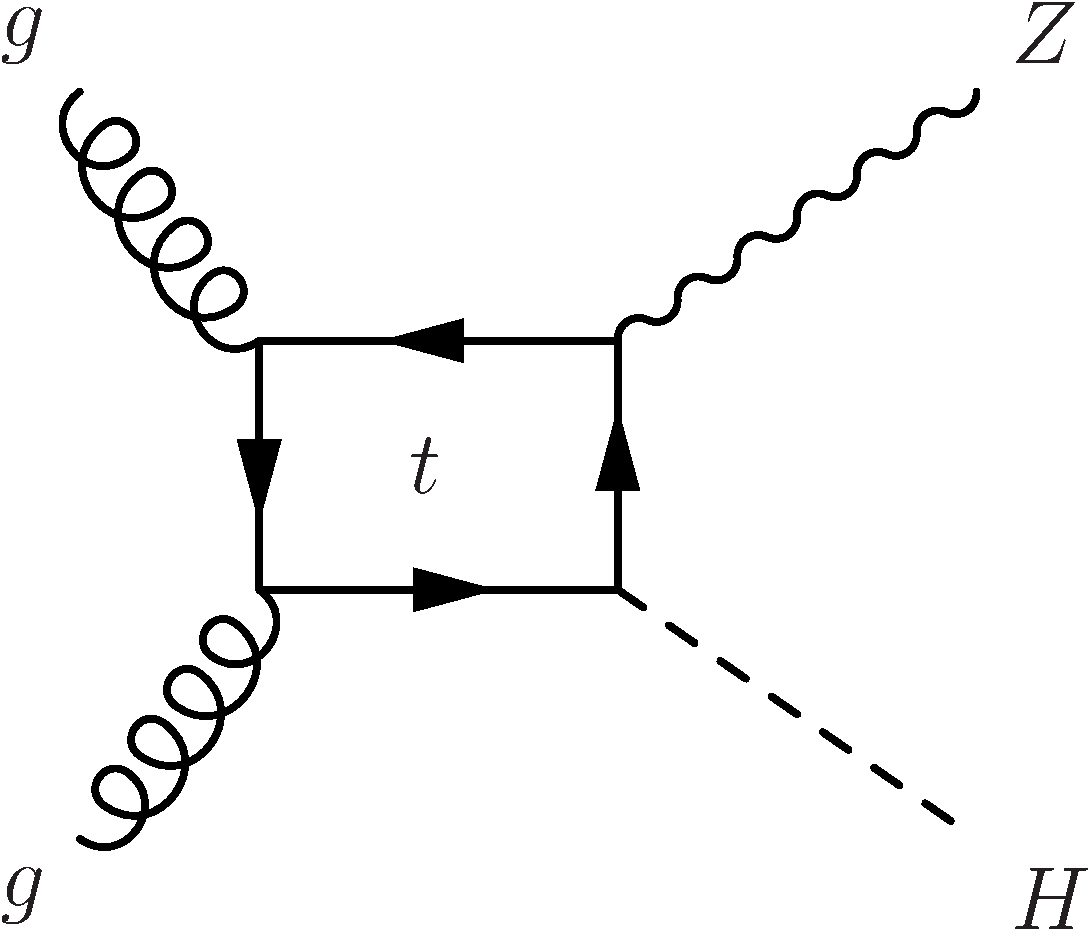
\includegraphics[scale=0.2]{images/production-ggZHbox_v2}} \qquad
    \subfigure [] {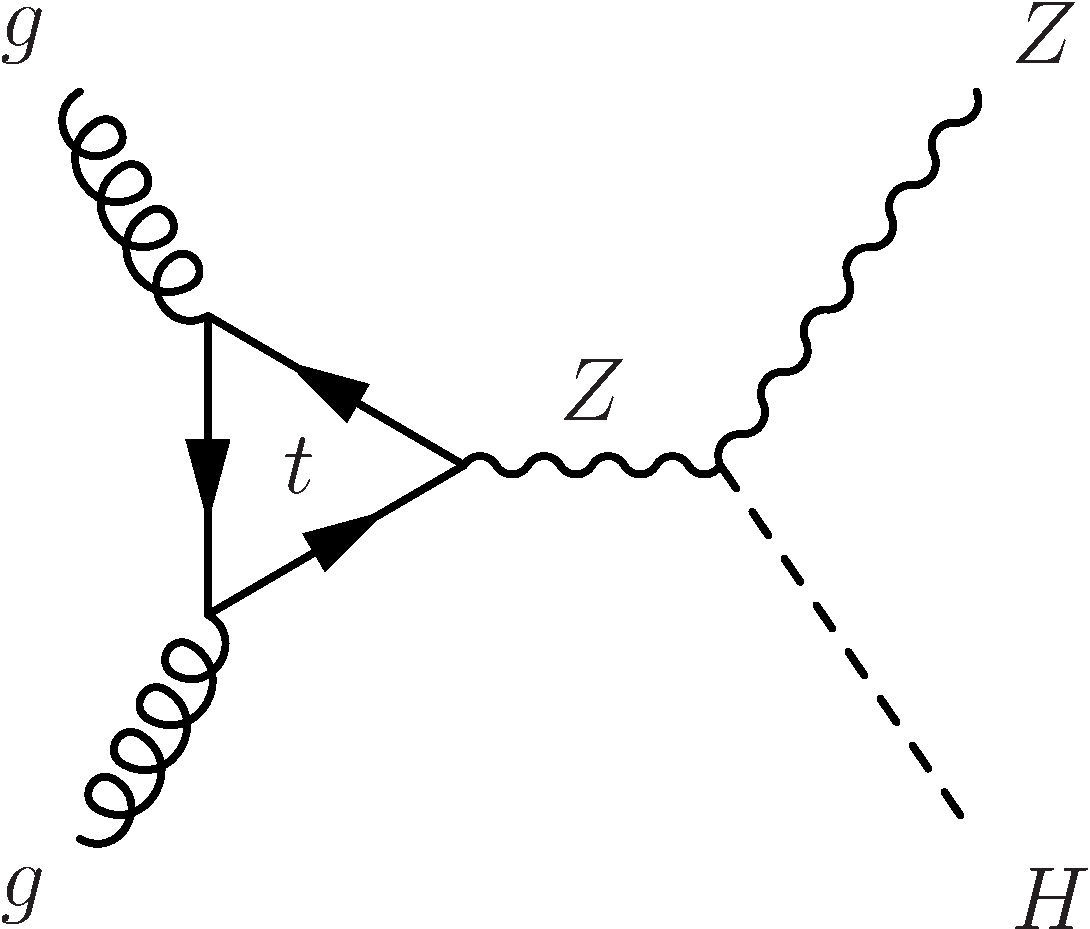
\includegraphics[scale=0.2]{images/production-ggZH}} \qquad
  }
  \caption[Higgs Boson Production Diagrams]{The Feynman diagrams for the Higgs boson production processes of A) gluon fusion; B) vector boson fusion; C) top quark pair associated production; D) vector boson associated production; E), D) top-loop induced contributions to the \bosZ\ boson associated production.}
  \label{fig:higgsprodfeyn}
\end{figure}

For the current center-of-mass energy of proton collisions at the LHC, $\sqrt{s} = 13\ \TeV$, and a Higgs boson mass of $\massH = 125\ \GeV$, the state-of-the-art values computed for the production cross sections\footnote{The cross sections are presented in units of picobarns $(\pb)$, where $1\ \mathrm{barn} = 10^{-24}\ \mathrm{cm}^{2}$.} are
\begin{alignat*}{2}
  &\sigma\left( pp \rightarrow H \right) &&= 48.58\ {}_{-6.7\%}^{+4.6\%} \ (\mathrm{theory}) \pm 3.2\%\ (\mathrm{PDF} + \alpha_{s})\ \pb, \\
  &\sigma\left( pp \rightarrow qqH \right) &&= 3.782\ {}_{-0.3\%}^{+0.4\%} \ (\mathrm{QCD\ scale}) \pm 2.1\%\ (\mathrm{PDF} + \alpha_{s})\ \pb, \\
  &\sigma\left( pp \rightarrow WH \right) &&= 1.373\ {}_{-0.7\%}^{+0.5\%} \ (\mathrm{QCD\ scale}) \pm 1.9\%\ (\mathrm{PDF} + \alpha_{s})\ \pb,
\end{alignat*}
\begin{alignat*}{2}
  &\sigma_{\mathrm{total}}\left( pp \rightarrow ZH \right) &&= 0.8839\ {}_{-3.1\%}^{+3.8\%} \ (\mathrm{QCD\ scale}) \pm 1.6\%\ (\mathrm{PDF} + \alpha_{s})\ \pb, \\
  &\sigma\left( gg \rightarrow ZH \right) &&= 0.1227\ {}_{-18.9\%}^{+25.1\%} \ (\mathrm{QCD\ scale}) \pm 2.4\%\ (\mathrm{PDF} + \alpha_{s})\ \pb, \\
  &\sigma\left( pp \rightarrow ttH \right) &&= 0.5071\ {}_{-9.2\%}^{+5.8\%} \ (\mathrm{QCD\ scale}) \pm 3.6\%\ (\mathrm{PDF} + \alpha_{s})\ \pb.
\end{alignat*}
The uncertainties are due to variations on the QCD renormalization scale ($\mathrm{QCD\ scale}$), the parton distribution function (PDF) that determines the momenta of the interacting partons, and the strong coupling constant ($\alpha_{s}$). The accuracy of these cross sections are determined by the inclusion of higher-order terms during their calculation, which is generally next-to-next-to-leading (NNLO) order in QCD and next-to-leading (NLO) in electroweak corrections. The exceptions are that the gluon fusion cross section is calculated further to N3LO in QCD, hence acquiring additional theoretical uncertainties, and the top quark pair associated production cross section which is calculated only to NLO in QCD. The methods and theoretical treatment of these cross section calculations are thoroughly documented in Ref. \cite{CERNYR4}.

\subsubsection{Decay Modes}

With a predicted lifetime\footnote{The total decay width of the Higgs boson is predicted to be $\Gamma_{H} = 4.088$ \MeV\ and the lifetime of a particle is given by $\tau = \hslash\ /\ \Gamma$.} of $1.6 \times 10^{-22}\ \mathrm{s}$, the Higgs boson decays almost immediately and its presence can only be inferred from its decay products. Based on its predicted properties, the final state of its decay must be electrically and color neutral. By conservation of mass, it must also decay into lighter particles so, for example, a decay into a top quark-antiquark pair $t\bar{t}$ is forbidden for low mass Higgs bosons. However, because the Higgs boson couples to particles in proportion to their masses, the heaviest allowed decays will be the most favored.

\begin{figure}[htbp]
  \centering
    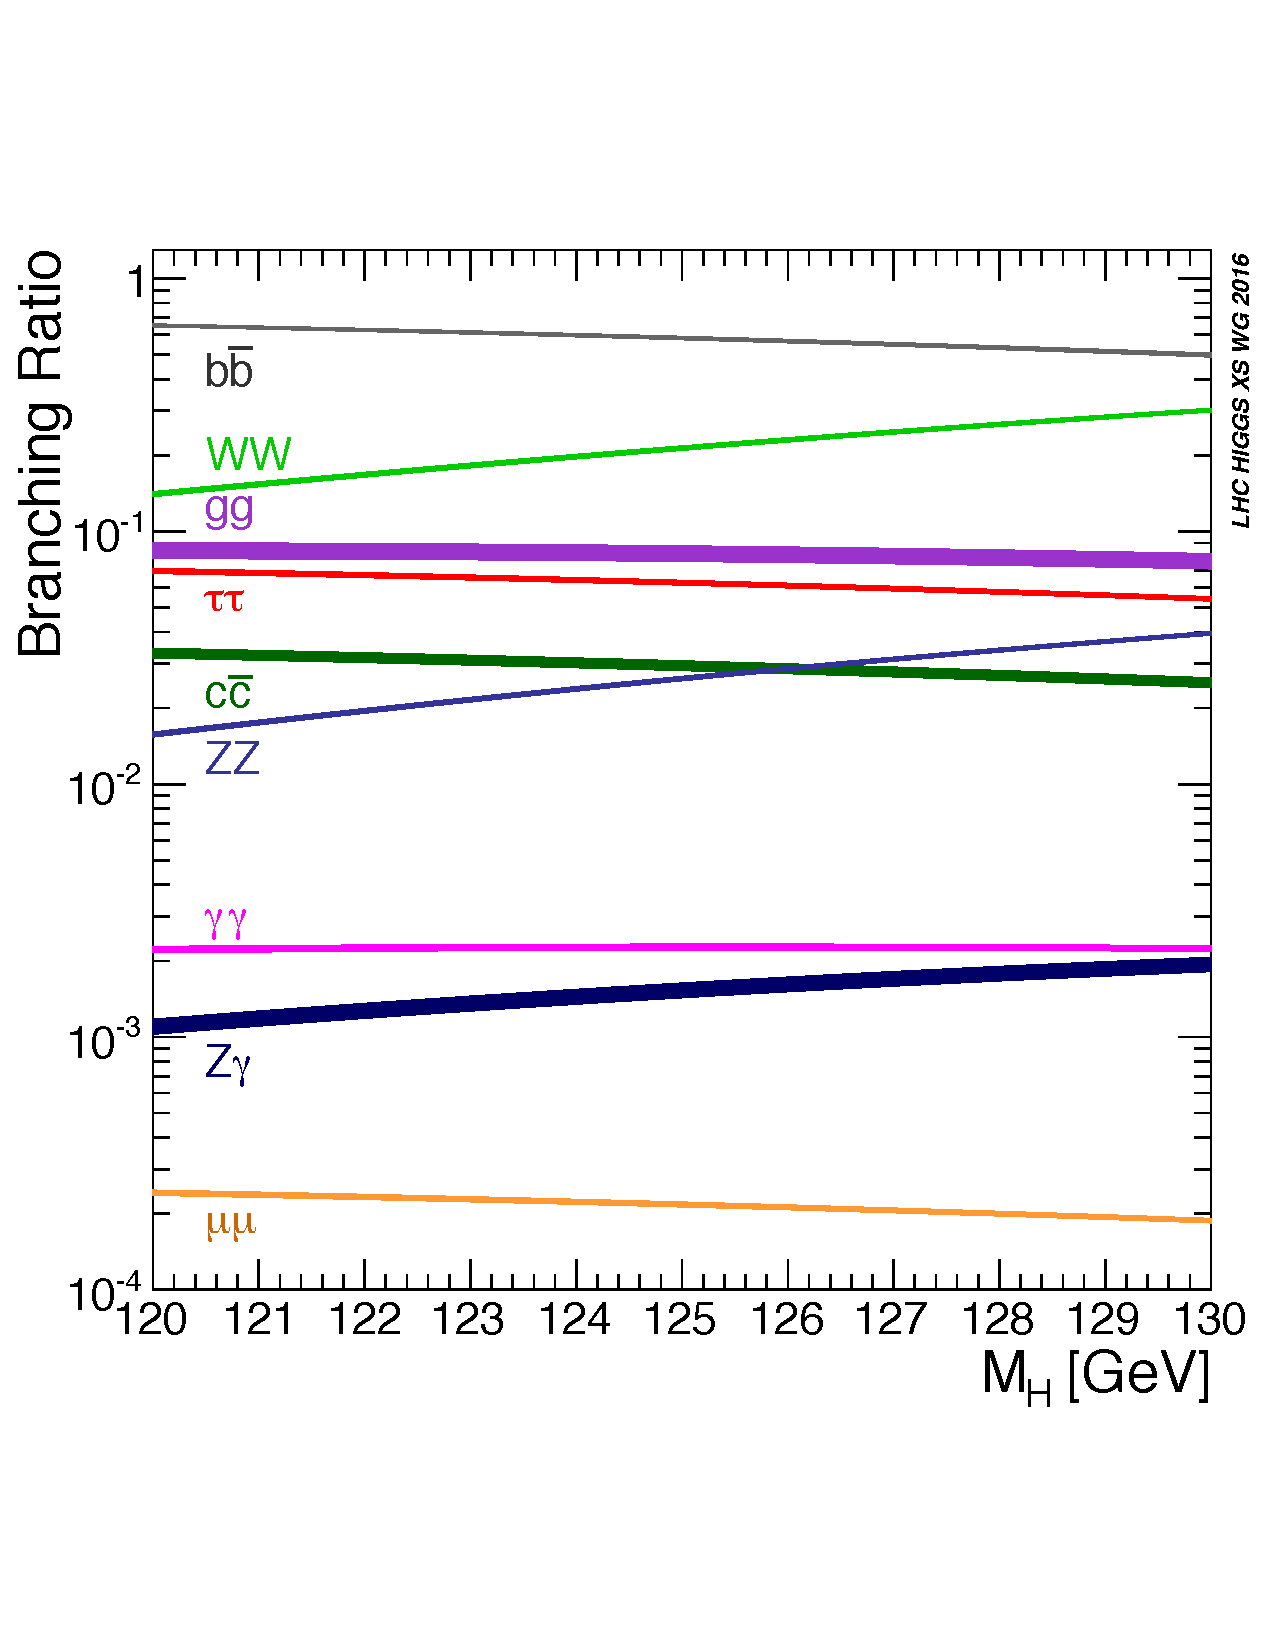
\includegraphics[width=3.5in]{images/SMHiggsBR-YR4-square}
    \caption[Higgs Boson Branching Ratios]{The branching ratios of the Higgs boson as a function of its mass \massH. \cite{CERNYR4}. The shaded bands indicate the theoretical uncertainty of the calculation while the labels indicate the decay mode.}
    \label{fig:higgsbrplots}
\end{figure}

The probability of a particular decay mode occuring is given by its \textit{branching ratio}, and is shown in Figure \ref{fig:higgsbrplots} as a function of the Higgs boson mass \massH. For a Higgs boson mass of $\massH = 125\ \GeV$, the state-of-the-art values computed for the branching ratios of its allowed decays are, in descending order,
\begin{alignat*}{2}
  &\textrm{BR}\left( H \rightarrow \bb \right) &&= 0.5824\ {}_{-0.65\%}^{+0.65\%}\ (\mathrm{theory}) {}_{-0.74\%}^{+0.72\%}\ (m_{q}) {}_{-0.80\%}^{+0.78\%}\ (\alpha_{s}), \\
  &\textrm{BR}\left( H \rightarrow \bosW\bosW \right) &&= 0.2137\ {}_{-0.99\%}^{+0.99\%}\ (\mathrm{theory}) {}_{-0.98\%}^{+0.99\%}\ (m_{q}) {}_{-0.63\%}^{+0.66\%}\ (\alpha_{s}), \\
  &\textrm{BR}\left( H \rightarrow \bosgln\bosgln \right) &&= 0.08187\ {}_{-3.41\%}^{+3.40\%}\ (\mathrm{theory}) {}_{-1.13\%}^{+1.12\%}\ (m_{q}) {}_{-3.61\%}^{+3.69\%}\ (\alpha_{s}), \\
  &\textrm{BR}\left( H \rightarrow \tau\bar{\tau} \right) &&= 0.06272\ {}_{-1.16\%}^{+1.17\%}\ (\mathrm{theory}) {}_{-0.98\%}^{+0.98\%}\ (m_{q}) {}_{-0.62\%}^{+0.62\%}\ (\alpha_{s}), \\
  &\textrm{BR}\left( H \rightarrow c\bar{c} \right) &&= 0.02891\ {}_{-1.20\%}^{+1.20\%}\ (\mathrm{theory}) {}_{-0.98\%}^{+5.26\%}\ (m_{q}) {}_{-1.25\%}^{+1.25\%}\ (\alpha_{s}), \\
  &\textrm{BR}\left( H \rightarrow \bosZ\bosZ \right) &&= 0.02619\ {}_{-0.99\%}^{+0.99\%}\ (\mathrm{theory}) {}_{-0.98\%}^{+0.99\%}\ (m_{q}) {}_{-0.63\%}^{+0.66\%}\ (\alpha_{s}), \\
  &\textrm{BR}\left( H \rightarrow \bosg\bosg \right) &&= 0.002270\ {}_{-1.72\%}^{+1.73\%}\ (\mathrm{theory}) {}_{-0.99\%}^{+0.93\%}\ (m_{q}) {}_{-0.62\%}^{+0.61\%}\ (\alpha_{s}), \\
  &\textrm{BR}\left( H \rightarrow \bosZ\bosg \right) &&= 0.001533\ {}_{-5.71\%}^{+5.71\%}\ (\mathrm{theory}) {}_{-1.01\%}^{+0.98\%}\ (m_{q}) {}_{-0.65\%}^{+0.58\%}\ (\alpha_{s}), \\
  &\textrm{BR}\left( H \rightarrow \mu\bar{\mu} \right) &&= 0.0002176\ {}_{-1.23\%}^{+1.23\%}\ (\mathrm{theory}) {}_{-0.99\%}^{+0.97\%}\ (m_{q}) {}_{-0.64\%}^{+0.59\%}\ (\alpha_{s}).
\end{alignat*}
The theoretical uncertainties account for missing higher-order QCD and electroweak corrections, while the parametric uncertainties cover the variations of the quark masses $m_{q}$, where $q = c,\ b,\ t$, and the strong coupling constant $\alpha_{s}$ which are input parameters to the calculation. The methods and theoretical treatment of the computation of these branching ratios is also documented in Ref. \cite{CERNYR4}.

\subsection{Discovery}

The discovery of a new boson with a mass close to 125 \GeV\ was announced on July 4, 2012 at CERN, with independent observations achieved by the ATLAS\cite{ATLASHiggsDiscovery} and CMS\cite{CMSHiggsDiscovery} collaborations. Within a year's time, the new particle would be verified by both experiments to have zero spin and positive parity\cite{ATLASHiggsVerify,CMSHiggsVerify} and its observed couplings would remain consistent with a Standard Model Higgs boson.\cite{HiggsCouplingConstraints} At this point, the new boson was recognized as a Higgs boson, and in 2013 the Nobel Prize in Physics would be awarded to Fran\c{c}ois Englert and Peter Higgs for their discovery of the Higgs mechanism and prediction of a Higgs boson almost half a century before its discovery.

The decay channels with the highest sensitivities were $\bosH \rightarrow \bosZ\bosZ$, with each \bosZ\ boson subsequently decaying into a pair of charged leptons, and $\bosH \rightarrow \bosg\bosg$, for which ATLAS and CMS both had observed local significances above the expected background of $3\sigma$ and $4\sigma$, respectively. While those channels individually passed the $3\sigma$ threshold for establishing evidence, it would take their combination with other channels for ATLAS to surpass and CMS to reach $5\sigma$, the threshold for declaring a discovery. By the beginning of 2015, when the LHC would resume operations since its first planned maintainence period, the Higgs production modes of gluon fusion and vector boson fusion had been observed, as well as its decays to $WW$, $ZZ$, and $\bosg\bosg$. 

\section{Searches for \VHbb}

The preferred decay mode of the Higgs boson, as determined by its measured mass of $\massH = 125.26 \pm 0.16\ \GeV$\cite{PDG2018}, is to a bottom quark-antiquark pair, henceforth \Hbb, with a branching ratio of nearly 59\%. An observation would establish clearly the coupling of the Higgs boson to bottom quarks, and to down-type quarks in general. Moreover, as the dominant decay mode, a precise measurement of its branching ratio has direct ramifications for improving the constraints on the total decay width of the Higgs boson and provides an opportunity to check for anomalous Yukawa couplings that may present a case for new physics beyond the Standard Model. The observation of \Hbb\ is therefore of great scientific interest and experiments must be dedicated towards searching for this decay.

\subsection{Motivation for \VHbb}

The experimental challenge of searching for \Hbb\ is in distinguishing its decay signature, or signal, from the immense background of Standard Model processes. The bottom and antibottom quarks produced by the decay will both hadronize due to color confinement, forming two unstable B-hadrons that subsequently decay into cones of lighter particles known as jets. Such a final state is not unique, as QCD processes which produce many jets are a common occurance. However, even if the pair of jets can be correctly identified as originating from bottom quarks and not lighter quarks or gluons, the multijet production of a bottom quark-antiquark pair occurs at a rate that is seven orders of magnitude greater than the gluon fusion production of a Higgs boson that decays into a bottom quark-antiquark pair, as shown in Figure \ref{fig:MCFM}. While advances in the field of jet substructure may eventually enable such a strategy\cite{ggHbb}, a direct search for final states containing only two \qrkb-jets faces a large and irreducible multijet background.

One solution for mitigating the multijet background is search for \Hbb\ using the remaining Higgs boson production modes and exploiting their final state topologies. The vector boson fusion final state is fully hadronic, as the two scattering quarks will form their own jets, and is challenging in its own right. The top-quark associated production final state potentially contains leptons from the dominant decay of the top quark, $\qrkt \rightarrow \bosW\qrkb$, but a combinatorial complexity arises with the presence of additional \qrkb-jets. The key lies in using the weak vector boson associated production mode, henceforth \VHbb, which offers a final state that can be distinguished by the leptonic decays of either the \bosW\ or \bosZ and thereby enabling the reduction of the multijet background to negligible levels.

\begin{figure}[htbp]
  \centering
    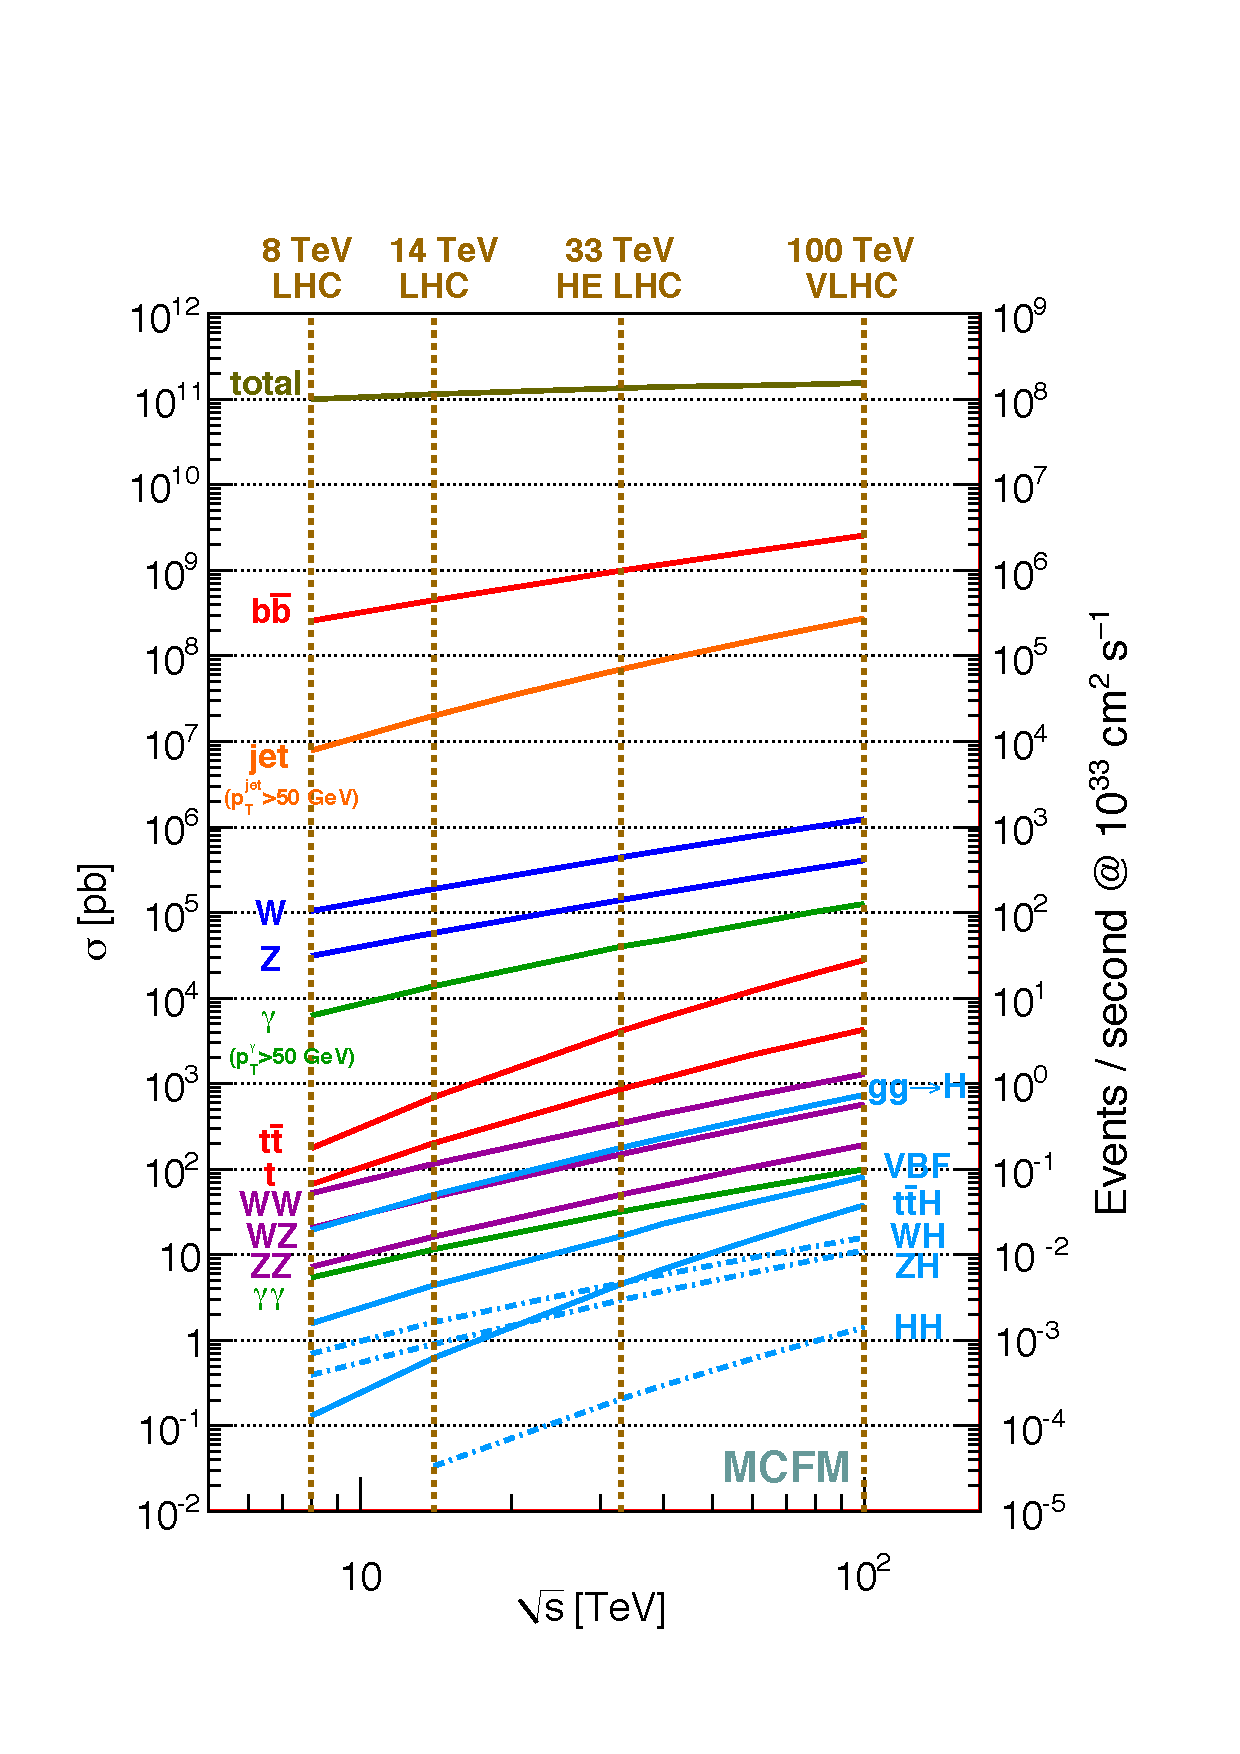
\includegraphics[width=3.5in]{images/mcfm-Edep}
    \caption[Production Cross Sections at the LHC]{The predicted production cross sections of various processes for the range of center-of-mass energies achieved and within reach at the LHC.\cite{MCFM}}
    \label{fig:MCFM}
\end{figure}

Searches based on \VHbb\ must also contend with known Standard Model background processes, such as those measured in Figure \ref{fig:SMxsec},  which mimic its final states. The main irreducible backgrounds come from \bosW\ and \bosZ\ bosons produced in association with jets, or $\bosV+\textrm{jets}$, and the production of top quark-antiquark pairs, or $t\bar{t}$, which have cross sections that are three to four orders of magnitude larger than that of \VHbb. The single top and diboson, or $\bosV\bosV$, processes are also important backgrounds, but with cross sections that are only one to two orders of magnitude larger than that of \VHbb. The Feynman diagrams for examples of these background processes are shown in Figure \ref{fig:VHbkgdiagrams}.

\begin{figure}[htbp]
  \centering
    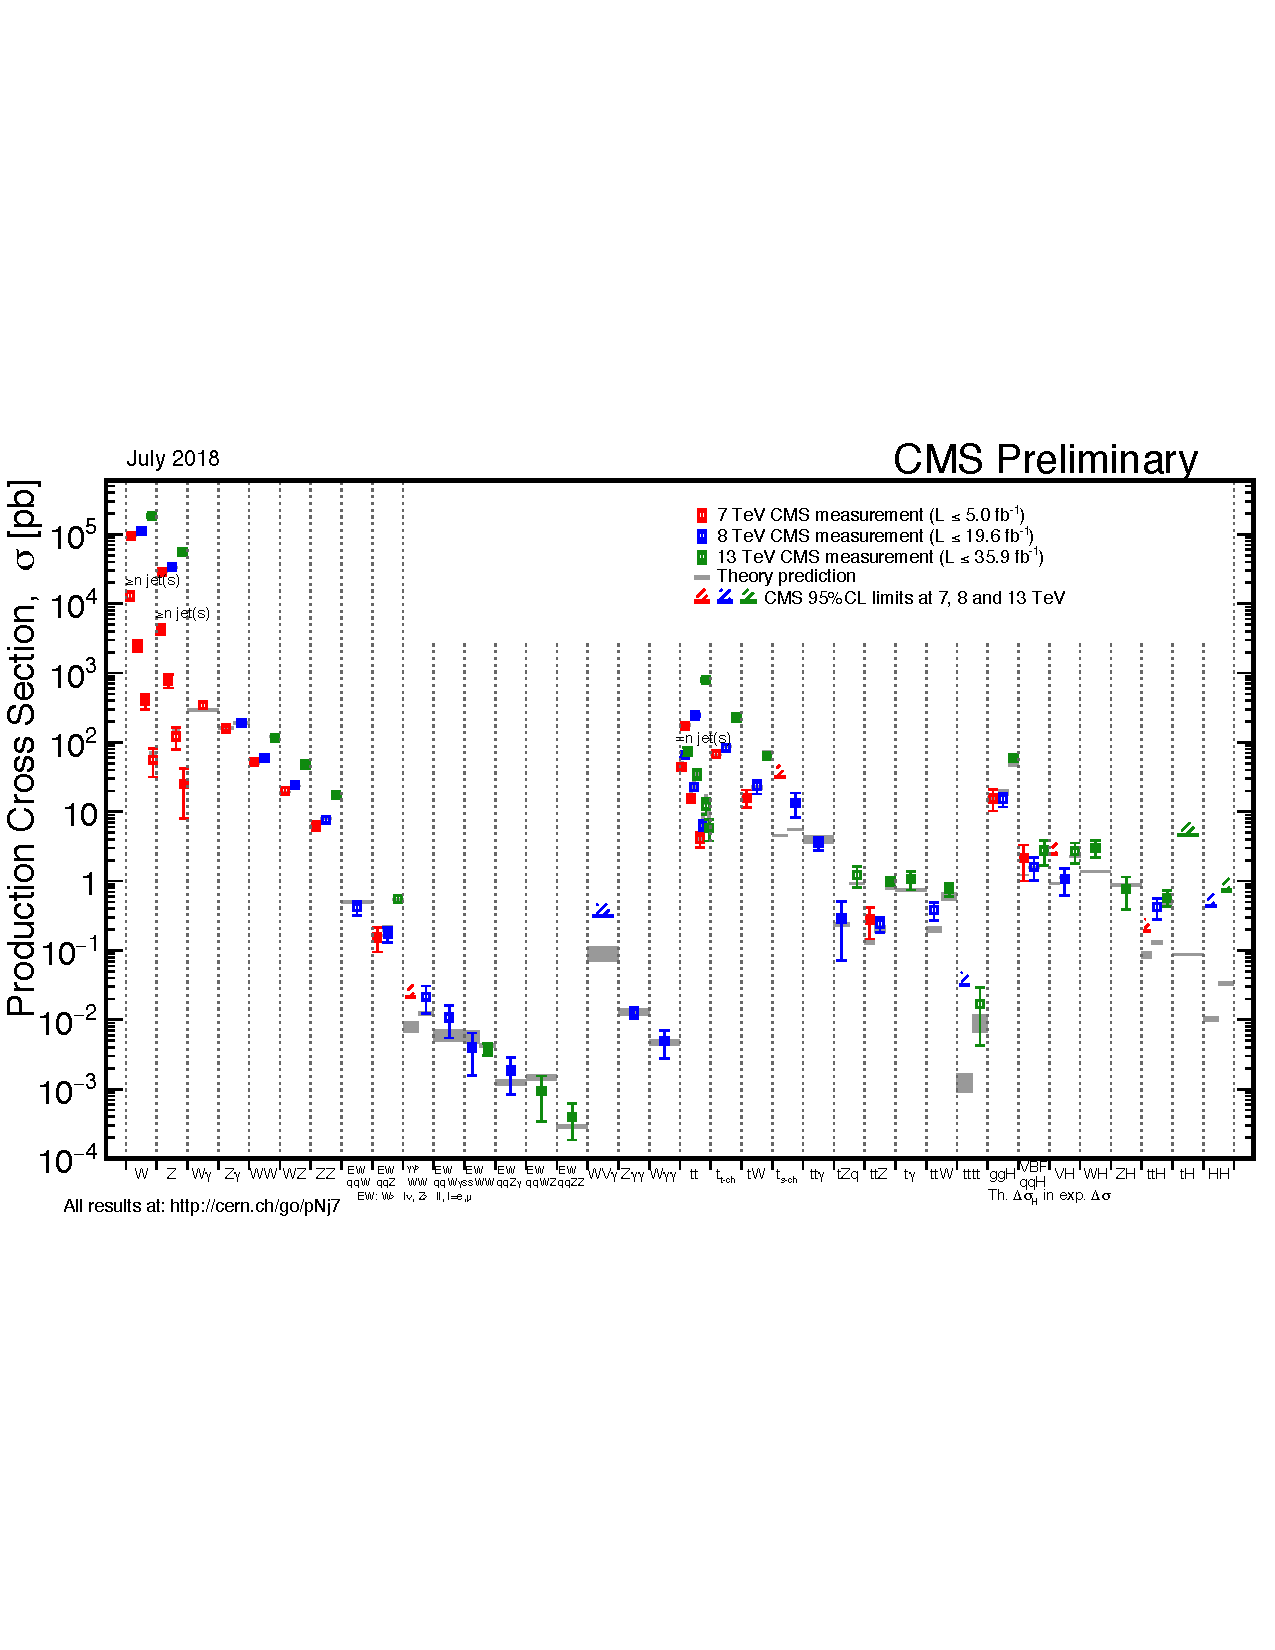
\includegraphics[width=6in]{images/SigmaNew_v0}
    \caption[CMS Measurements of SM Production Cross Sections]{Measurements of the production cross sections of the Standard Model processes by the CMS experiment.\cite{CMSSMXSEC}. The agreement with prediction holds remarkably well across the different center-of-mass energies of collisions at the LHC.}
    \label{fig:SMxsec}
\end{figure}

\begin{figure}[htbp]
  \centering
  \mbox{
    \subfigure [] {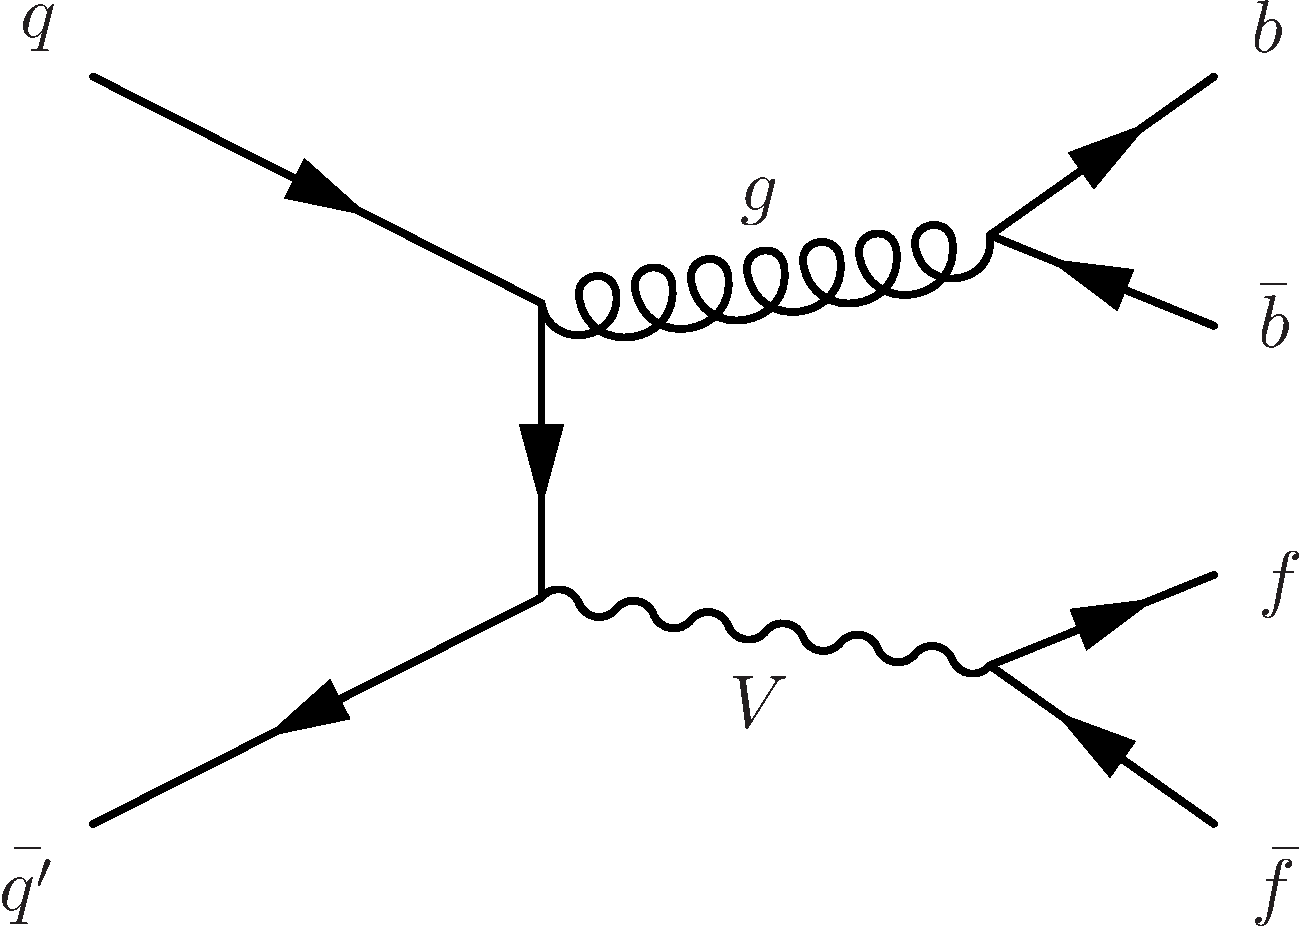
\includegraphics[scale=0.2]{images/background-Vjets}} \qquad
    \subfigure [] {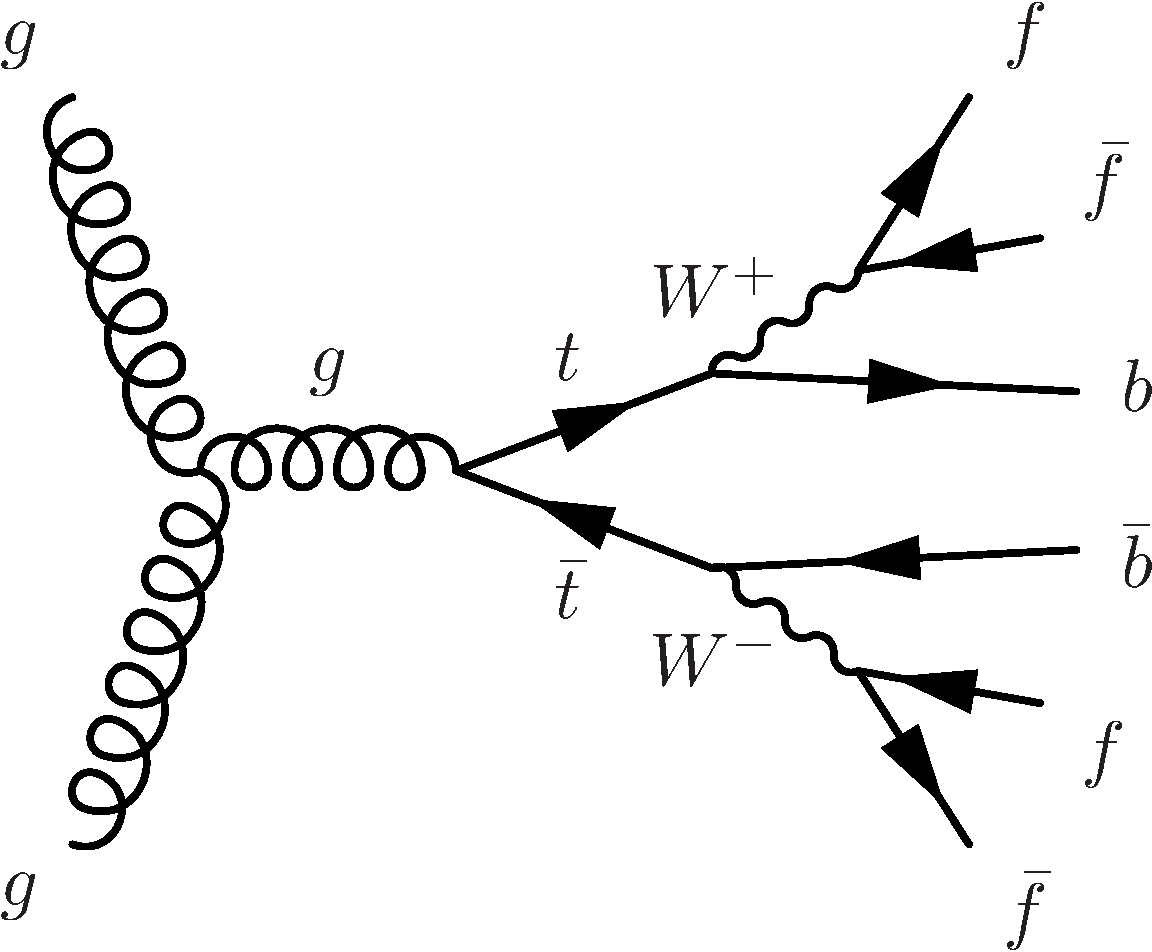
\includegraphics[scale=0.2]{images/background-tt}} \qquad
  }
  \mbox{
    \subfigure [] {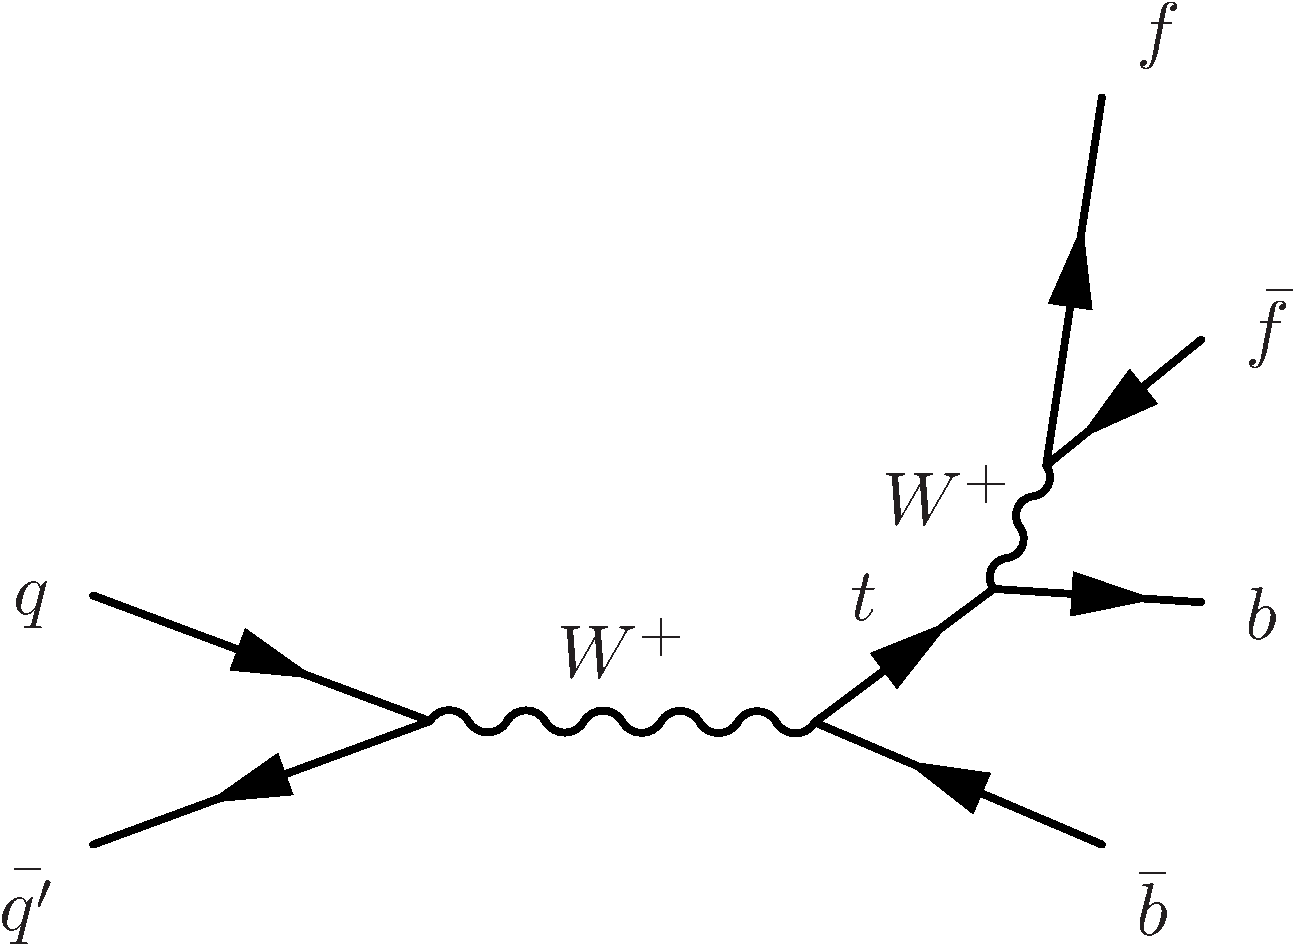
\includegraphics[scale=0.2]{images/background-top}} \qquad
    \subfigure [] {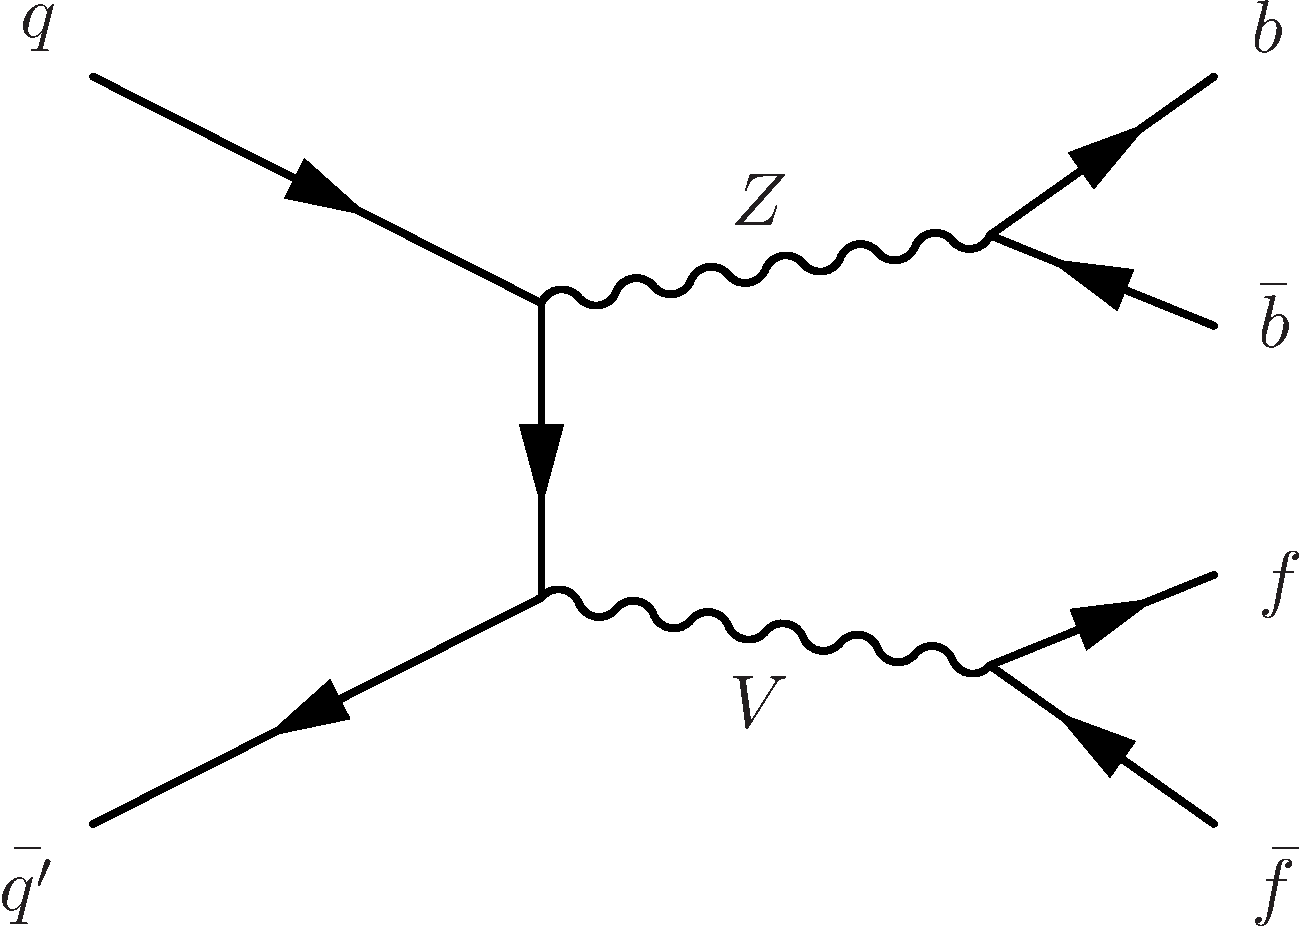
\includegraphics[scale=0.2]{images/background-VV}} \qquad
  }
  \caption[\VHbb\ Background Process Diagrams]{The Feynman diagrams for the Standard Model background processes to \VHbb. A) vector boson production in associated with jets ($\bosV+\textrm{jets}$); B) top quark-antiquark pair production ($t\bar{t}$); C) single top  D) diboson ($\bosV\bosV$).}
  \label{fig:VHbkgdiagrams}
\end{figure}

\subsection{Previous Results}

The first searches for \VHbb\ coincided with the first searches for the Higgs boson and began at the Large Electron-Positron (LEP) collider which operated from 1989 to 2000 at CERN in Geneva, Switzerland. There a Higgs boson would have been produced primarily through \bosZ\ boson associated production initiated by the annihilation of the electron and positron. Although the Higgs boson was not found, the four LEP experiments ALEPH, DELPHI, OPAL, and L3 analyzed the full dataset collected at center-of-mass energies above $\sqrt{s} = 189\ \GeV$\ and established a lower bound of 114.4 \GeV\ for the mass of the Higgs boson at the 95\% confidence level.\cite{LEPResult}

The first searches for \VHbb\ using hadron collisions were done at the Tevatron at Fermi National Accelerator Laboratory (FNAL) in Batavia, Illinois. The Tevatron collided protons and antiprotons at center-of-mass energies up to $\sqrt{s} = 1.96\ \TeV$\ and operated from 1985 until 2011. Although the Higgs boson was not observed, a combined analysis of the full Tevatron datasets collected by the CDF and D0 experiments yielded an observed significance of $2.8\sigma$, just shy of establishing evidence for the \VHbb\ decay.\cite{TevatronResult}

The most recent searches for \VHbb\ have taken place at the Large Hadron Collider (LHC), also located at CERN, using collisions between protons. During Run 1, which lasted from 2010 to 2013, the LHC collided protons at center-of-mass energies of $\sqrt{s} = 7\ \mathrm{and}\ 8\ \TeV$. Analysis of the Run 1 datasets were unable to obtain evidence for \VHbb\, with observed significances of $1.4\sigma$ and $2.5\sigma$ by the ATLAS and CMS experiments, respectively.\cite{ATLASVHbbRun1,CMSVHbbRun1} A combination of these results only brought the observed significance up to $2.6\sigma$.\cite{ATLASandCMSVHbbRun1}

After its upgrades during Long Shutdown 1 (LS1), the LHC resumed operations and Run 2 commenced with the center-of-mass energy of collisions increased to $\sqrt{s} = 13\ \TeV$. Although the increase in energy meant a larger cross section for \VHbb, it also led to relatively larger increases in the cross sections of the Standard Model background processes as demonstrated in Table \ref{tbl:SvsBxsec}, further complicating the search for \VHbb. However, this pessimism was unwarranted, as ATLAS and CMS both established evidence for the \VHbb\ decay by observing significances of $3.6\sigma$ and $3.8\sigma$, respectively, after combining the results of their initial Run 2 and Run 1 analyses.

\begin{table}[htbp]
  \caption[Production Cross Sections for the Higgs Boson and SM Background Process at the LHC]{A list of Higgs boson and Standard Model background production cross sections at center-of-mass energies of $\sqrt{s} = 8\ \mathrm{and}\ 13\ \TeV$, along with the relative increase at $\sqrt{s} = 13\ \TeV$.}
  \label{tbl:SvsBxsec}
  \begin{tabularx}{6.5in}{XXXX}
    \hline
    Cross Section                                  & $\sqrt{s} = 8\ \TeV$ & $\sqrt{s} = 13\ \TeV$ & Relative Increase at $\sqrt{s} = 13\ \TeV$ \\
    \hline
    $\sigma\left( pp \rightarrow H \right)$        & 19.4 \pb             & 44.1 \pb              & 2.27                                       \\
    $\sigma\left( pp \rightarrow qqH \right)$      & 1.6 \pb              & 3.8 \pb               & 2.38                                       \\
    $\sigma\left( pp \rightarrow VH \right)$       & 1.23 \pb             & 2.26 \pb              & 1.84                                       \\
    $\sigma\left( pp \rightarrow ttH \right)$      & 133 \fb              & 507 \fb               & 3.81                                       \\
    $\sigma\left( pp \rightarrow t\bar{t} \right)$ & 253 \pb              & 832 \pb               & 3.29                                       \\
    \hline
  \end{tabularx}
\end{table}

Naive projections assuming increased statistics and similar systematic uncertainties suggested that an observation of \VHbb\ may be possible if the experimental sensitivty could be improved by about 20\%. With Run 2 on track to produce more data in 2017 than 2016, such a historic result appeared to be on the horizon. The analysis of the 2017 dataset and the results obtained by the CMS experiment are the subject of this dissertation.

%We don't make the Chapter titles in All Caps Automatically because it is easier for you to type your Chapter Titles in uppercase than for those that need to have mixed case in their titles to find the correct command in the ufthesis.cls file and change it there. \renewcommand*{\thefootnote}{\fnsymbol{footnote}}\footnote{an un-numbered footnote - this is how you tell the readers that this chapter was previously published and then cite the Journal where it was published} We don't recommend that you change much of anything in the class file unless you're absolutely sure of what your are doing.\renewcommand*{\thefootnote}{\arabic{footnote}}\setcounter{footnote}{0}\footnote{and now we're back to normal footnote marking}

%Title case is where all principal words are capitalized except prepositions, articles, and conjunctions.  %\cite{green2008wrinkle}

%\subsection{Subsection Commands Are Also in Title Case}
%The difference, of course, are the second level headings are left-aligned
%
%\subsubsection{Subsubsections are in sentence case}
%The third level subheadings are left-aligned but in sentence case. Only the first letter and any proper nouns are capitalized. %\cite{strickler1998contamination}
%
%\subsubsection{If you divide a section, you must divide it into two, or more, parts}
%
%{\bf Paragraph headings.} There is no official fourth level heading. Do not use the Paragraph heading feature in LaTeX, simply apply the bold characteristic to the first few words of a paragraph followed by a colon or period.

%\subsection{I Need Another Second Level Heading in This Section}
%
%Aliquam mi nisi, tristique at rhoncus quis, consectetur non mi. Phasellus blandit quam ligula, a viverra lacus commodo at. In iaculis nisl vel pretium sollicitudin. In efficitur massa vel elit sollicitudin, vel auctor sapien cursus. Proin feugiat sapien a mi tempus;
%
% $ X-X'=D+D'$
%
% in consequat augue cursus. Nulla sed sagittis purus. Nunc eu consequat orci, eu laoreet enim. Ut euismod tincidunt sem, eget lacinia dui luctus eu. Aliquam mi augue, faucibus id semper vitae, porta ac ligula. Morbi sed ultrices odio. Mauris id luctus ex. Nulla ac libero dictum, interdum turpis lacinia, scelerisque leo. Praesent varius orci ac eros varius pharetra.
%
%\section{Image Handling in XeLaTeX}
%
%One of the biggest reasons for switching from the dvipdfm/dvipdfmx methods of compiling is the improved image handling capabilities. EPS, Bit-mapped, PDF, JPG, and PNG formats work well with the xelatex process.
%
%\subsection{The Traditional EPS Format}
%
%EPS format is the traditional format for LaTeX, but EPS files can be very large and many programs can't create or view these images. There are many programs that are used to interpret data and output the results as an EPS format image. It has been my experience that there are bounding box problems with these figures. On many occasions we have opened the image in Adobe Photoshop and, without making any changes, saved the document as a Photoshop EPS file, re-compiled the document, and the image worked correctly, so if you are having problems with an EPS image not showing in your document correctly, try this fix first.
%
%
%\begin{figure}[htbp]
%  \centering
%    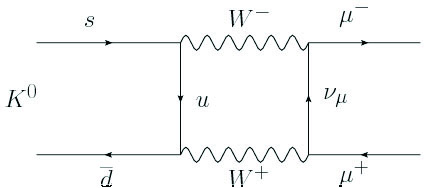
\includegraphics[width=5in]{images/diagram}
%    \caption[EPS format diagram. Note: no filetype is designated by adding an extension.]{EPS format diagram. Note: no filetype is designated by adding an extension. The file type is determined and the correct procedure is automatically chosen by xelatex.}
%\end{figure}
%
%
%Quisque malesuada a leo eget ullamcorper. Curabitur ut aliquam quam. Nam quis quam id mauris aliquam blandit porttitor sit amet quam. Donec ut erat eleifend turpis finibus pulvinar.
%
%\subsection{Bitmapped Images Work As Well}
%
%Bitmapped images are a standard file type on PCs, but these files are also usually very large so compressed images may be a better alternative.
%
%\begin{figure}[htbp]
%  \centering
%    \includegraphics[width=5in]{images/eagle}
%    \caption[BMP format drawing. Note: no filetype is designated by adding an extension.]{BMP format drawing. Note: no filetype is designated by adding an extension. The file type is determined and the correct procedure is automatically chosen by xelatex.}
%\end{figure}
%
%Morbi hendrerit risus nec quam posuere viverra. Donec quis tellus faucibus, molestie arcu sed, congue urna. Duis eget neque ac libero pulvinar porta eget et magna. Donec a magna eu eros suscipit cursus ac vitae nisl. Vivamus ligula purus, congue sed tortor blandit, ultrices egestas nisl.
%
%\subsection{Not to Mention PDF}
%
%It is often very handy to be able to include a pdf file as an image. By using XeLaTeX this is usually just matter of setting the size, or scale properties correctly.
%
%\begin{figure}[htbp]
%  \centering
%    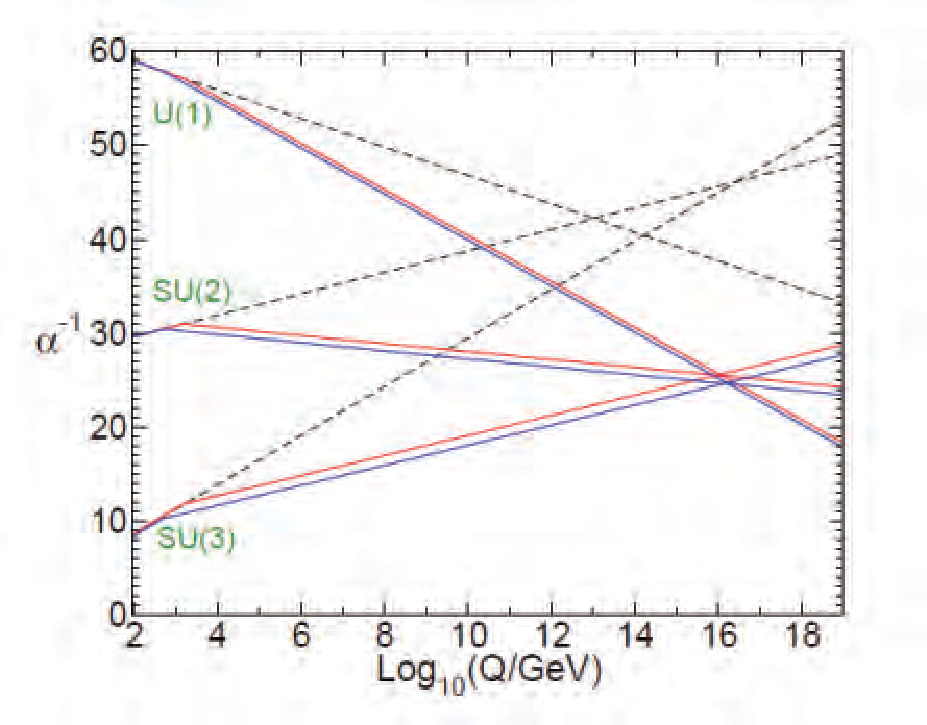
\includegraphics[scale=1.0]{images/graph.pdf}
%    \caption[PDF format graph. Note: no filetype is designated by adding an extension.]{PDF format graph. Note: no filetype is designated by adding an extension. The file type is determined and the correct procedure is automatically chosen by xelatex.}
%\end{figure}
%
%Nulla mattis augue lacus. Nam non lectus dolor. Cras ac quam vel justo elementum vestibulum. Integer vulputate pulvinar lacus sit amet pulvinar.
%
%\subsection{JPG Is Absolutely Necessary}
%
%For photographs, JPG is the most common format. This format is a fraction of the size of Bit-mapped images and can deliver very good quality at a much smaller overhead. Vestibulum eu lectus vel orci dictum vehicula. Proin id maximus dolor. Integer augue ante, pulvinar ac erat vitae, porttitor ullamcorper libero. %\cite{l2012wrinkle}
%
%\begin{figure}[htbp]
%  \centering
%    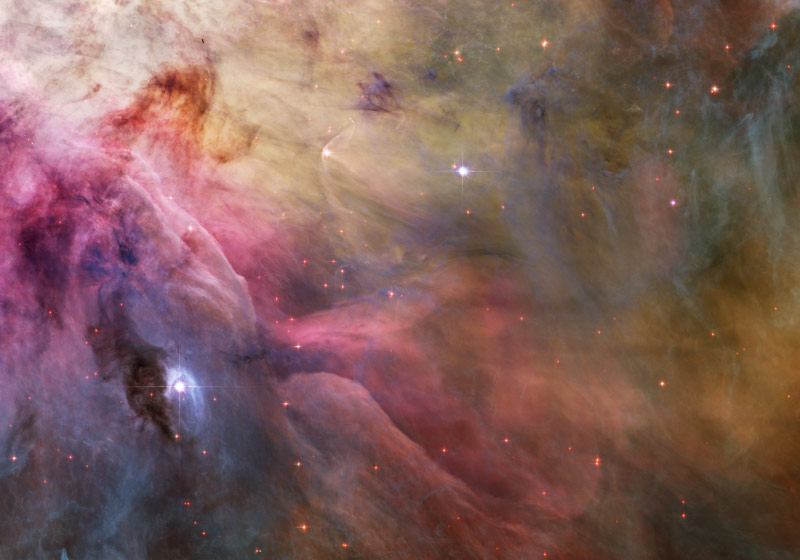
\includegraphics[width=5in]{images/nebula}
%    \caption[JPG format image. Note: no filetype is designated by adding an extension.]{JPG format image. Note: no filetype is designated by adding an extension. The file type is determined and the correct procedure is automatically chosen by xelatex.}
%\end{figure}
%
%Nunc blandit scelerisque velit, ac facilisis dui finibus et. Sed facilisis tortor vel commodo luctus. Donec est felis, malesuada id nibh in, accumsan malesuada lectus. Sed lobortis volutpat felis, vitae aliquet augue congue id. Fusce ut odio tincidunt, condimentum nulla vel, pharetra arcu.
%
%\subsection{PNGs Will Help Make Files Smaller}
%
%PNG files are even smaller than JPGs and are very good when text and images are combined.
%
%\begin{figure}[htbp]
%  \centering
%    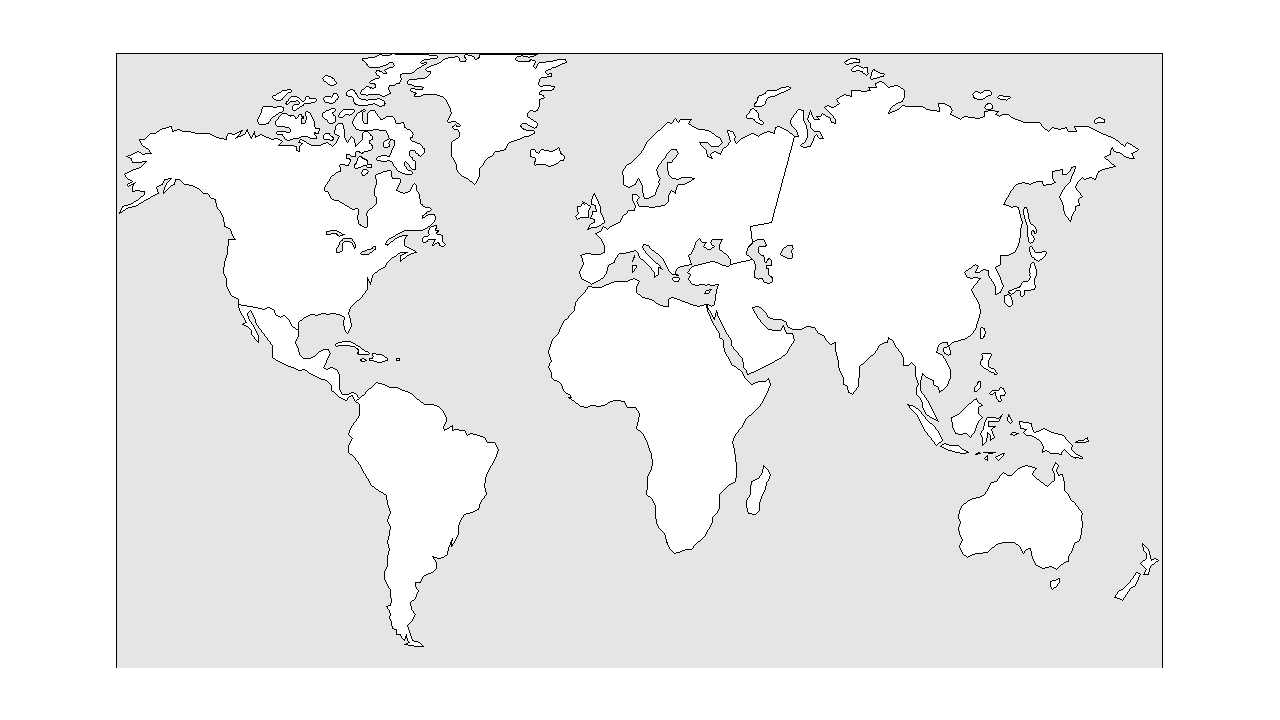
\includegraphics[width=5in]{images/theworld}
%    \caption[PNG format map. Note: no filetype is designated by adding an extension.]{PNG format map. Note: no filetype is designated by adding an extension. The file type is determined and the correct procedure is automatically chosen by xelatex.}
%\end{figure}
%
%
%
%Aenean condimentum libero sed mi porta, tempus ullamcorper lectus venenatis. Aliquam in diam dolor. Maecenas tempus consectetur sem et pulvinar. Aenean aliquam at metus ut hendrerit. Vivamus molestie ac neque eu luctus. Nam convallis maximus quam non lobortis. Fusce sit amet lorem et massa convallis aliquet at sit amet nulla. Suspendisse nec ex elit. Aenean gravida, sapien vitae congue commodo, urna turpis ornare libero, at cursus risus libero in erat. %\cite{Rust94}
%
%\section{GIF, TIF, and Others}
%
%Other file formats have not been successful, with or without file extensions. The tests have not been exhaustive so if you have a different type, give it a try. GIF, and TIF both do NOT work at this time. The next image demonstrates how to use multiple images as a single figure. Notice, there is a single caption for ALL figures and that caption starts with a discription of the ENTIRE figure before breaking off into the subfigure descriptions.
%
%\begin{figure}[htbp]
%     \centering
%   \mbox{
%      \subfigure [] {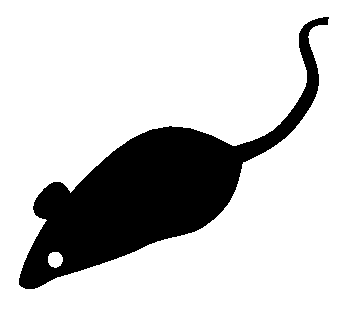
\includegraphics[scale=0.6]{images/mouse}} \qquad
%      \subfigure []{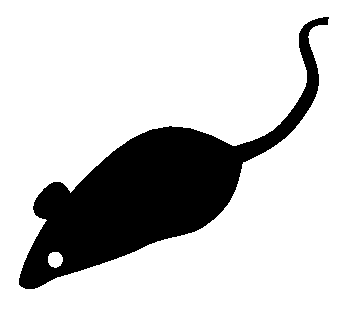
\includegraphics[scale=0.6]{images/mouse}} \qquad
%     }
%    \mbox{
%      \subfigure [] {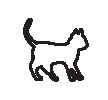
\includegraphics[scale=3]{images/cat}} \qquad
%      \subfigure [] {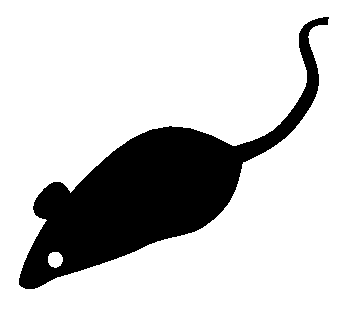
\includegraphics[scale=0.6]{images/mouse}} \qquad
%      }
%    \caption[Tom and Jerry]{Tom and Jerries. This caption demonstrates how the sub-captions are left out of the List of Figures, but included in the figure itself. A) Tom the first; B) Tom the second; C) Jerry; D) Tom the third.}
%    \label{mice}
%  \end{figure}
%
%
%Aliquam mi nisi, tristique at rhoncus quis, consectetur non mi. Phasellus blandit quam ligula, a viverra lacus commodo at. In iaculis nisl vel pretium sollicitudin. In efficitur massa vel elit sollicitudin, vel auctor sapien cursus. Proin feugiat sapien a mi tempus, in consequat augue cursus. Nulla sed sagittis purus. Nunc eu consequat orci, eu laoreet enim. Ut euismod tincidunt sem, eget lacinia dui luctus eu. Aliquam mi augue, faucibus id semper vitae, porta ac ligula. Morbi sed ultrices odio. Mauris id luctus ex. Nulla ac libero dictum, interdum turpis lacinia, scelerisque leo. Praesent varius orci ac eros varius pharetra.
%
%
%
%Nunc blandit scelerisque velit, ac facilisis dui finibus et. Sed facilisis tortor vel commodo luctus. Donec est felis, malesuada id nibh in, accumsan malesuada lectus.
%\begin{itemize} %
%    \item WinEDT: This text editor is recommended for use editing \TeX-files as it has many useful built in macros and is easy to use  %
%    \item This program can be found and downloaded here: \url{http://www.winedt.com/} %
%    \item The GIMP (GNU Image Manipulation Program) %
%    \begin{itemize}%
%        \item A freeware graphics editing program for picture editing and file conversions %\vspace{-12pt}%
%        \item Comparable to Adobe Photoshop %\vspace{-12pt}%
%        \item Can be downloaded here: \url{http://www.gimp.org/}%
%    \end{itemize}
%    \item A good reference of \LaTeX 2\ensuremath{\epsilon} commands%
%    \begin{itemize}
%        \item This should be included on the ETD website here: \url{http://etd.helpdesk.ufl.edu/tex.php}
%    \end{itemize}
%\end{itemize} %
%
%
%Sed lobortis volutpat felis, vitae aliquet augue congue id. Fusce ut odio tincidunt, condimentum nulla vel, pharetra arcu. In ultricies libero diam, nec rutrum magna vehicula nec. Praesent dictum eros sit amet turpis ultricies, eleifend condimentum dui imperdiet. Donec congue urna ante, id rutrum mi commodo a. Vivamus id tincidunt nunc. Morbi id lacus ut augue ultricies convallis. Duis a lectus quis ante pretium scelerisque nec nec nisi. In id porta justo, at euismod diam. Suspendisse vel tempus arcu. Praesent vel cursus nisi, ac rhoncus odio.

